\documentclass[journal]{IEEEtran}

\usepackage[utf8]{inputenc}
\usepackage[T1]{fontenc}
\usepackage{amsmath,amssymb}
\usepackage{graphicx}
\usepackage{booktabs}
\usepackage{multirow}
\usepackage{array}
\usepackage{siunitx}
\usepackage{xspace}
\usepackage{cite}
\usepackage{url}
\usepackage[hidelinks]{hyperref}

\graphicspath{{figures/}}

% Shared notation, used by every section.
\newcommand{\mapfifty}{mAP@50\xspace}
\newcommand{\mapfiftyninetyfive}{mAP@50--95\xspace}
\newcommand{\armA}{Arm~A (defaults)\xspace}
\newcommand{\armB}{Arm~B (random search)\xspace}
\newcommand{\armC}{Arm~C (PSO)\xspace}
\newcommand{\genone}{Generation~1\xspace}
\newcommand{\gentwo}{Generation~2\xspace}

\begin{document}

\title{SwarmSort: A Fair Evaluation of Particle Swarm Hyperparameter Optimization for YOLOv8 Waste Detection Across Studio, Real-World, and Indian Data}

\author{Shreyansh~Jain%
\thanks{S. Jain is with the Department of Computer Science and Engineering, Netaji Subhas University of Technology (NSUT), New Delhi, India.}}

\markboth{}{Jain: SwarmSort}

\maketitle

\begin{abstract}
Waste sorting needs detectors that find every item in a photograph, yet much published work classifies single objects on studio backgrounds, and metaheuristic tuning claims rarely include a random-search baseline or confidence intervals. We ask whether particle swarm optimization (PSO) trains a better lightweight waste detector than random search or library defaults at an equal budget. Six training hyperparameters of YOLOv8n were set by the defaults, the best of 32 random samples, or 8 particles over 4 rounds, each search spending 32 short proxy trainings; a check fixed in advance confirmed the proxy ranks settings like longer training (Spearman correlation 0.976, first generation). Each chosen setting was trained and tested once on held-out data, with paired-bootstrap 95\% confidence intervals. The first generation used studio images; the second added real-world photographs and a test-only Indian street set. On studio data, defaults, random search and PSO tie at 0.676, 0.672 and 0.668 mean average precision at intersection-over-union 0.5 (\mapfifty). With real-world training data, both searches significantly beat the defaults on the mixed test set (by 0.017 and 0.020 \mapfifty) but not each other; on real-world photographs (0.298--0.310) no difference is significant, and Indian photographs score only 0.023--0.027. On the same test images, real-world training data raised real-world \mapfifty from 0.038--0.096 to 0.338--0.353 and cost 0.074--0.105 on studio images, all significantly. The optimizer matters little and the data matter most; tuning claims need equal-budget random-search baselines and confidence intervals.
\end{abstract}

\begin{IEEEkeywords}
Waste detection, particle swarm optimization, hyperparameter optimization, YOLOv8, random search, real-world generalization, India.
\end{IEEEkeywords}


\section{Introduction}
\label{sec:intro}

\IEEEPARstart{W}{aste} can be recycled, composted or safely disposed of only if its materials are kept apart. India's Solid Waste Management Rules, 2016 require every waste generator to segregate waste at source into bio-degradable, non-bio-degradable and domestic hazardous streams (Rule~4), with green, white and black bins for bio-degradable, recyclable and other waste (Rule~15(h))~\cite{moefcc2016solid}. A camera that names each item's material could support this segregation at a smart bin, sorting line or collection point, and artificial intelligence is already an established tool in solid waste management~\cite{abdallah2020artificial,fang2023artificial}.

In the literature we reviewed, however, most vision work on waste sorting solves an easier problem: classifying one photograph of one object, often on a plain background, as with TrashNet~\cite{yang2016classification} and its classifiers~\cite{kaya2023classification}. A heap, a conveyor or a street holds many items, some touching or partly hidden, and each must be located as well as named: an object-detection task. Majchrowska et al.~\cite{majchrowska2022deep}, the starting point of this work, localize litter with one network and classify each detected crop with another. Multi-object waste detection is thus established, but it is a smaller strand than single-object classification, and several detection studies still rely on single-object studio images: the task and scene gap (G1).

Detectors are also sensitive to training hyperparameters such as the learning rate, momentum, weight decay and augmentation strength; the TrashNet authors blamed the 22\% test accuracy of their convolutional neural network (CNN) on unsuitable hyperparameters~\cite{yang2016classification}. Metaheuristics have tuned CNNs, for example particle swarm optimization (PSO)~\cite{kennedy1995particle} for a mammography classifier~\cite{aguerchi2024cnn} and a beluga whale optimizer for an InceptionV3 waste classifier~\cite{sayed2024intelligent}, but the evidence is weaker than the reported gains suggest. In the studies we reviewed, metaheuristic tuning in waste vision targeted classifiers, and no waste detector had its training hyperparameters tuned by a swarm optimizer (G2). Tuned models were compared with other metaheuristics or with nothing, not with random search~\cite{bergstra2012random} at the same number of evaluations, and test results were single numbers without confidence intervals (G3), so a gain cannot be credited to the optimizer's guidance rather than to the search effort itself.

The data are a second weakness. Reviews find many waste-sorting vision studies set in simplified environments with artificially collected data~\cite{lu2022computer} that differ from real waste~\cite{fang2023artificial}, and accuracy depends heavily on the dataset: the same YOLOv5x, trained and tested on each dataset separately, scored 84.9 AP$_{50}$ on PlastOPol but 63.3 on TACO~\cite{cordova2022litter}. A tuning gain on studio images may thus say little about street photographs. For India, where segregation at source is mandatory, the closest resource, the Dense Waste Segmentation Dataset (DWSD)~\cite{ali2025dwsd}, reports segmentation pixel accuracy only, and we found no Indian real-world waste test set with published object-detection baselines (G4).

SwarmSort tests the tuning question under strict conditions. It trains YOLOv8n~\cite{jocher2023ultralytics}, a nano detector small enough for a smart bin or a phone, and compares three ways (arms) of choosing six of its training hyperparameters: the library defaults (Arm~A), the best of 32 random samples (Arm~B) and a hand-written PSO with 8 particles over 4 rounds (Arm~C). Both searches spend 32 short proxy trainings. Each chosen setting is trained once for 100 epochs and tested once on a held-out split, with paired-bootstrap 95\% confidence intervals on every difference. \genone used studio-style images in six classes; \gentwo added real-world photographs, a seventh class (OTHER) and a test-only Indian set built from DWSD. We address three research questions:
\begin{enumerate}
\item[RQ1:] At an equal budget of 32 proxy trainings, does PSO find YOLOv8n training hyperparameters that beat random search and the default settings on a held-out test set? (G2, G3)
\item[RQ2:] Does a short proxy training (12 epochs on 40\% of the data) rank hyperparameter settings the same way longer training does? (G3)
\item[RQ3:] Does the answer to RQ1 change when the data move from studio images to real-world and Indian scenes, and how large is the studio-to-real-world drop? (G1, G4)
\end{enumerate}

Our contributions are as follows.
\begin{itemize}
\item \textit{A lightweight multi-object waste detector} (G1): YOLOv8n trained on multi-object studio and real-world scenes, with six classes in \genone and seven in \gentwo (Sections~\ref{subsec:datasets} and~\ref{subsec:detector}).
\item \textit{A swarm-tuned waste detector} (G2): a hand-written PSO searches the learning-rate schedule, momentum, weight decay and two augmentation settings (Sections~\ref{subsec:space} and~\ref{subsec:pso}); to our knowledge, within the literature we reviewed, no earlier waste detector had its training hyperparameters tuned by a swarm optimizer.
\item \textit{An equal-budget, three-arm protocol} (G3): a proxy-validity check with a pass threshold fixed in advance, passed with Spearman $\rho = 0.976$ ($n = 8$, \genone only), a test split used once and paired-bootstrap 95\% confidence intervals on every difference (Sections~\ref{subsec:design}, \ref{subsec:proxy} and~\ref{subsec:eval}).
\item \textit{A two-generation evaluation across domains} (G4): studio, real-world and Indian results reported separately, including detection results on DWSD, which, to our knowledge, within the literature we reviewed, had no published detection baselines. Our DWSD boxes come from mask regions that merge touching items, and the class mapping was inferred from the masks, so these results also measure a labeling mismatch. On the same test images, real-world training data raised real-world \mapfifty from 0.038--0.096 (\genone) to 0.338--0.353 (\gentwo), at a cost of 0.074--0.105 on studio images, all significant (Section~\ref{subsec:res-domain}).
\item \textit{An honest answer, with null results reported} (O5): PSO never meaningfully beat random search; its only significant edge, $+0.003$ \mapfifty on the Indian set, lies on scores near zero. Tuning gains over the defaults were absent in \genone, small in \gentwo ($+0.017$ and $+0.020$ on the mixed test set) and did not reach real-world or Indian photographs. We explain these results (Section~\ref{sec:discussion}) and release the code, search logs, result files and trained models.
\end{itemize}

Section~\ref{sec:related} reviews related work and derives gaps G1--G4, Section~\ref{sec:methods} describes the methods, and Section~\ref{sec:results} answers RQ2, RQ1 and RQ3, in that order. Section~\ref{sec:discussion} discusses the results, their implications and the limitations, Section~\ref{sec:future} gives a prioritized roadmap, and Section~\ref{sec:conclusion} concludes.

\section{Related Work and Research Gaps}
\label{sec:related}

\section{Materials and Methods}
\label{sec:methods}

Each design choice answers a gap of Section~\ref{subsec:gaps}: a multi-object detector instead of a classifier (G1), a swarm optimizer applied to a detector's training hyperparameters (G2), an equal-budget comparison with random search and the defaults, judged with confidence intervals on a test split used once (G3), and separate studio, real-world and Indian test sets (G4).

\subsection{Experimental Design}
\label{subsec:design}

Three arms choose the training hyperparameters of one detector (Fig.~\ref{fig:pipeline}). \armA uses the Ultralytics defaults without search and is the reference any tuning must beat; \armB takes the best of 32 random samples, and \armC the best setting found by a particle swarm of 8 particles over 4 rounds. Both search arms score candidates with the same proxy training (Section~\ref{subsec:proxy}), so the budget is counted in proxy trainings, not in wall-clock time, which varied between methods and cloud sessions (Section~\ref{subsec:res-cost}). Each arm's chosen setting is trained once with an identical recipe (Section~\ref{subsec:training}) and scored once on a held-out test split (Section~\ref{subsec:eval}).

The experiment was run twice. \genone uses one studio-style dataset with six classes at 416~px; \gentwo adds real-world training photographs, a seventh class (OTHER), 640~px images and a test-only Indian set. Search space, PSO settings, seeds, recipes and evaluation code are shared, and both searches were rerun from scratch. Since classes, image size and training data differ, the two generations' scores are not one benchmark; their dedicated comparison is described in Section~\ref{subsec:eval}.

\begin{figure}[!t]
\centering
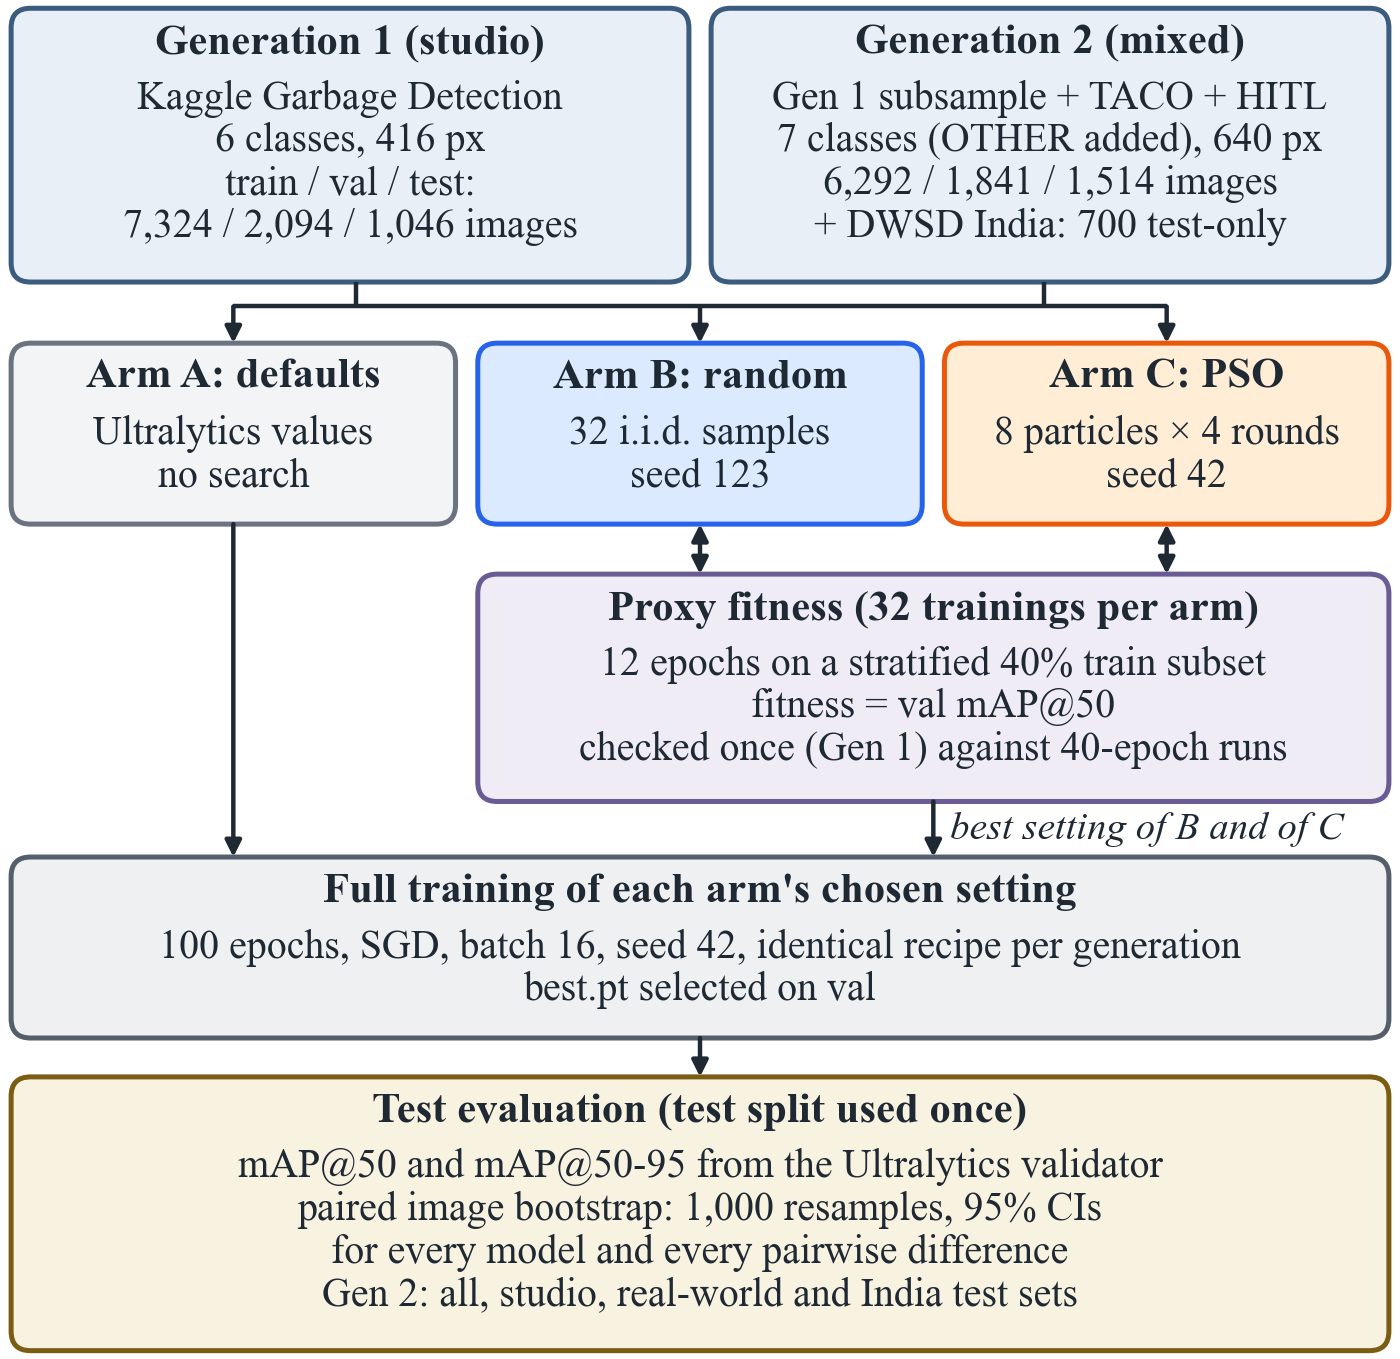
\includegraphics[width=\columnwidth]{m_pipeline.png}
\caption{Experimental pipeline shared by both generations. Arms~B and~C each spend 32 proxy trainings; Arm~A uses the library defaults without search. Each arm's chosen setting is trained once for 100 epochs and tested once.}
\label{fig:pipeline}
\end{figure}

\subsection{Datasets}
\label{subsec:datasets}

Table~\ref{tab:datasets} lists every source with its licence and split sizes.

\textit{\genone data.} The Kaggle dataset ``Garbage Detection -- 6 Waste Categories''~\cite{viswaprakash2024garbage}, from a Roboflow project, holds studio-style images with YOLO boxes in six classes: BIODEGRADABLE, CARDBOARD, GLASS, METAL, PAPER and PLASTIC. In training, 36.45\% of the boxes cover less than 1\% of the image, and BIODEGRADABLE holds 61.92\% of the boxes against 5.61\% for PAPER. The provided folders are split by class (the validation folder has 13,632 BIODEGRADABLE but 33 PAPER boxes, the test folder no GLASS box), so we pooled all images and re-split them 70/20/10, stratified by source class (seed 42), with at least 30 boxes per class in validation and test. Near-duplicates stay in one split: images count as copies if their files are identical (MD5), share a Roboflow source image, or have 256-bit difference hashes within 10 bits, or within 40 bits with a Pearson correlation of at least 0.90 between $64\times64$ grayscale thumbnails. This found 47 groups (133 images). The label checks found 17 zero-size boxes and no corrupt or unlabeled image.

\textit{\gentwo training data.} \gentwo has seven classes: the six \genone classes, with unchanged indices, plus OTHER. A subsample of the \genone splits, stratified by dominant class (seed 42), keeps 3,000 training and 900 validation images, and all test images are kept, so the \gentwo studio test set is the \genone test set. TACO~\cite{proenca2020taco} adds crowd-sourced photographs of litter in the wild; all 60 categories were mapped (for example, drink cans to METAL, cigarettes to OTHER), giving 1,260 OTHER but only 8 BIODEGRADABLE boxes. The HITL Recycling dataset~\cite{hitl2026recycling} adds street photographs, almost all with one litter box, classed by the object tag where decisive (food waste $\to$ BIODEGRADABLE), otherwise by the material tag (aluminum $\to$ METAL), else OTHER; 100 objects lacked a material tag. TACO and HITL were split 70/20/10 with the same duplicate rules and stored with a long side of at most 640~px. The merged data have 962 duplicate groups, none spanning two sources or splits; 918 byte-identical pairs inside the real-world sources cause no leakage but give some photographs extra weight. BIODEGRADABLE holds 51.96\% of the training boxes and OTHER 3.89\%; the studio images have no OTHER box, and the real-world test set a single BIODEGRADABLE box.

\textit{Indian test set.} The Dense Waste Segmentation Dataset (DWSD)~\cite{ali2025dwsd} has 784 phone photographs of streets, parks and garbage areas in Kolkata and Berhampore, West Bengal, annotated as $448\times448$ semantic masks. We used it only for testing, never for training, search or model selection. Each 8-connected region of one mask value (of at least 50 pixels) became a box, so touching items of one class merge into one large box. The class mapping had to be inferred: the published table of mask values does not match what the regions show (the value listed as background covers polythene bags in 610 masks), so we named each value by inspecting its regions; six of the fifteen remain uncertain. The 84 images without boxes were excluded, as some show unannotated waste, leaving 3,040 PLASTIC, 1,230 PAPER, 124 CARDBOARD, 90 OTHER and 18 METAL boxes. An MD5 cross-check against the 9,647 main-build images found no identical file.

\begin{table*}[!t]
\centering
\caption{Datasets. Counts are images, with boxes in parentheses. ``Classes'' is the number of target classes that occur in the source. The \gentwo studio test set equals the \genone test set; the \gentwo real-world test set is the union of the TACO and HITL test images (468 images, 779 boxes).}
\label{tab:datasets}
\footnotesize
\setlength{\tabcolsep}{4pt}
\begin{tabular}{@{}llllllccc@{}}
\toprule
Generation & Source & Domain & Licence & Stored size & Classes & Train & Validation & Test \\
\midrule
\genone & Garbage Detection (Kaggle) & studio & CC BY 4.0 & $416\times416$ & 6 & 7,324 (51,756) & 2,094 (14,904) & 1,046 (7,413) \\
\midrule
\multirow{5}{*}{\gentwo} & \genone subsample & studio & CC BY 4.0 & $416\times416$ & 6 & 3,000 (22,206) & 900 (6,904) & 1,046 (7,413) \\
 & TACO~\cite{proenca2020taco} & real-world & CC BY 4.0 & long side $\le 640$ & 7 & 1,050 (3,293) & 301 (1,031) & 149 (460) \\
 & HITL Recycling & real-world & CC0 & long side $\le 640$ & 7 & 2,242 (2,246) & 640 (641) & 319 (319) \\
 & Total (7 classes) & mixed & & & 7 & 6,292 (27,745) & 1,841 (8,576) & 1,514 (8,192) \\
 & DWSD~\cite{ali2025dwsd} & India & CC BY 4.0 & $448\times448$ & 5 & -- & -- & 700 (4,502) \\
\bottomrule
\end{tabular}
\end{table*}

\subsection{Detector}
\label{subsec:detector}

All arms train YOLOv8n, the nano variant of the YOLOv8 single-stage detectors~\cite{redmon2016you,jocher2023ultralytics}, with Ultralytics 8.4.169, starting from COCO-pretrained weights~\cite{lin2014microsoft} with the class outputs resized to our six or seven classes. The nano model suits a smart bin or phone with limited compute and keeps 32 proxy trainings per arm affordable on one cloud GPU.

\subsection{Search Space}
\label{subsec:space}

Both search arms explore the same six dimensions (Table~\ref{tab:space}): the initial learning rate \texttt{lr0}, the final learning rate as a fraction of it (\texttt{lrf}), the SGD \texttt{momentum}, the \texttt{weight\_decay}, the probability of mosaic augmentation (\texttt{mosaic}) and the gain of random rescaling (\texttt{scale}). The optimizers work in ``search units'': \texttt{lr0} and \texttt{weight\_decay}, which span two orders of magnitude, are held as base-10 exponents (a particle at $-3.2$ means $\texttt{lr0}=10^{-3.2}$), the others as values; decoded values are rounded to six significant digits. Three defaults lie on the boundary, \texttt{lrf} on the lower bound and \texttt{lr0} and \texttt{mosaic} on the upper bounds, so the searches reach them only at the edge. All other training hyperparameters kept the library defaults in every arm.

\begin{table}[!t]
\centering
\caption{Search Space and Search Settings (Shared by Both Generations)}
\label{tab:space}
\footnotesize
\begin{tabular}{@{}p{0.27\columnwidth}lll@{}}
\toprule
Hyperparameter & Range & Scale & Default (Arm~A) \\
\midrule
\texttt{lr0} & $10^{-4}$ to $10^{-2}$ & $\log_{10}$ & 0.01 \\
\texttt{lrf} & 0.01 to 0.2 & linear & 0.01 \\
\texttt{momentum} & 0.60 to 0.98 & linear & 0.937 \\
\texttt{weight\_decay} & $10^{-5}$ to $10^{-3}$ & $\log_{10}$ & 0.0005 \\
\texttt{mosaic} & 0.0 to 1.0 & linear & 1.0 \\
\texttt{scale} & 0.2 to 0.8 & linear & 0.5 \\
\midrule
Setting & \multicolumn{3}{l@{}}{Value} \\
\midrule
PSO budget & \multicolumn{3}{p{0.63\columnwidth}@{}}{8 particles $\times$ 4 rounds $=$ 32 evaluations} \\
Inertia $w_t$ & \multicolumn{3}{p{0.63\columnwidth}@{}}{0.9, 0.65, 0.4 (linear over 3 update steps)} \\
$c_1$, $c_2$ & \multicolumn{3}{p{0.63\columnwidth}@{}}{1.5, 1.5} \\
$\mathbf{r}_1$, $\mathbf{r}_2$ & \multicolumn{3}{p{0.63\columnwidth}@{}}{$U(0,1)$, fresh per particle and dimension} \\
Velocity limit & \multicolumn{3}{p{0.63\columnwidth}@{}}{$\pm20\%$ of each range} \\
Initialization & \multicolumn{3}{p{0.63\columnwidth}@{}}{positions uniform in bounds; velocities uniform in $\pm10\%$ of each range} \\
Boundaries & \multicolumn{3}{p{0.63\columnwidth}@{}}{position clipped; velocity of a clipped dimension set to 0} \\
PSO seed & \multicolumn{3}{p{0.63\columnwidth}@{}}{42} \\
Random search & \multicolumn{3}{p{0.63\columnwidth}@{}}{32 i.i.d.\ uniform samples in search units; seed 123} \\
Fitness & \multicolumn{3}{p{0.63\columnwidth}@{}}{validation \mapfifty after a 12-epoch proxy training on a stratified 40\% training subset} \\
\bottomrule
\end{tabular}
\end{table}

\subsection{Particle Swarm Optimization}
\label{subsec:pso}

Arm~C uses a global-best particle swarm optimizer~\cite{kennedy1995particle} with an inertia weight~\cite{shi1998modified}, hand-written in NumPy, that maximizes the proxy fitness. Particle $i$ has a position $\mathbf{x}_i \in \mathbb{R}^6$ in search units, a velocity $\mathbf{v}_i$ and its best visited position $\mathbf{p}_i$; $\mathbf{g}$ is the swarm's best. One update step is
\begin{equation}
\mathbf{v}_i \leftarrow w_t\,\mathbf{v}_i + c_1\,\mathbf{r}_1 \odot (\mathbf{p}_i - \mathbf{x}_i) + c_2\,\mathbf{r}_2 \odot (\mathbf{g} - \mathbf{x}_i),
\label{eq:velocity}
\end{equation}
where $\odot$ is the element-wise product and $\mathbf{r}_1$, $\mathbf{r}_2$ are redrawn at every step (Table~\ref{tab:space}). Each component $v_{i,d}$ is then clamped to $[-v_{\max,d},\, v_{\max,d}]$ with $v_{\max,d} = 0.2\,(u_d - l_d)$, where $l_d$ and $u_d$ are the bounds of dimension $d$, and
\begin{equation}
\mathbf{x}_i \leftarrow \min\bigl(\max(\mathbf{x}_i + \mathbf{v}_i,\ \mathbf{l}),\ \mathbf{u}\bigr),
\label{eq:position}
\end{equation}
element-wise; a clipped dimension's velocity is set to zero, so the particle rests at the wall. Round~1 evaluates the random initial swarm, and each of the $T-1 = 3$ update steps is followed by one more round, so $T = 4$ rounds use exactly 32 evaluations. The inertia weight falls linearly,
\begin{equation}
w_t = w_{\mathrm{start}} - (w_{\mathrm{start}} - w_{\mathrm{end}})\,\frac{t-1}{T-2}, \qquad t = 1, \dots, T-1,
\label{eq:inertia}
\end{equation}
from $w_{\mathrm{start}} = 0.9$ to $w_{\mathrm{end}} = 0.4$. The inertia weight is the concept of~\cite{shi1998modified}; this linear schedule is our setting, chosen so that the swarm explores first and refines later. A personal best is replaced only by a strictly higher fitness. All randomness comes from one seeded generator, so an interrupted search resumes exactly by replaying the seed and the logged fitness values. A failed training (non-finite \mapfifty) would get fitness 0 and never be selected; none occurred in the four searches.

As a code check, with 20 particles, 50 rounds and 10 seeds on $[-5.12, 5.12]^6$, the median best value was $1.9\times10^{-5}$ on Sphere and 6.96 on the multimodal Rastrigin function (both with minimum 0): the optimizer converges on a smooth bowl and keeps improving among many local minima. This makes no claim about tuning performance.

\subsection{Random Search and Defaults}
\label{subsec:random}

Arm~B draws 32 points uniformly in search units (log-uniform for \texttt{lr0} and \texttt{weight\_decay}) and scores them with the same proxy and script as the swarm. Random search~\cite{bergstra2012random} is included because any structured optimizer should beat it at the same budget. Each search arm's winner is its highest proxy fitness (the first on a tie). Arm~A uses the defaults in Table~\ref{tab:space}.

\subsection{Proxy Fitness and Its Validation}
\label{subsec:proxy}

A full training takes over an hour on our GPU, so the searches score candidates with a 12-epoch proxy training on a stratified 40\% training subset: 2,930 of the 7,324 \genone images (by source class) and 40\% of the 6,292 \gentwo images (by source and dominant class). The subset is drawn once (seed 42) and stored as an image list, so every candidate trains on the same images. The fitness is the validation \mapfifty of the last-epoch weights. The proxy follows the full-training recipe (Section~\ref{subsec:training}), except that the no-mosaic period and the warm-up keep their share of the run, 10\% and 3\% (\texttt{close\_mosaic} 1 epoch, warm-up 0.36 epochs), which keeps the searched \texttt{mosaic} faithful to the full run.

Before the \genone searches, we tested whether the proxy ranks settings like a longer training. Seven configurations drawn by Latin hypercube sampling~\cite{mckay1979comparison} in search units (SciPy, ``random-cd'', seed 42) plus the defaults were each trained with the proxy and with a 40-epoch ``medium'' run on the full training split (\texttt{close\_mosaic} 4, warm-up 1.2 epochs), both at 416~px. The statistic was the Spearman rank correlation~\cite{spearman1904proof} of the eight score pairs; the pass threshold, $\rho \ge 0.6$, and the fallback, a 20-epoch proxy, were fixed in advance (results in Section~\ref{subsec:res-proxy}).

The check was not repeated for \gentwo; the decision, recorded before its searches, relied on the \genone result and the unchanged recipe, so proxy validity under the new data, classes and image size is assumed, not tested. The check also has only eight configurations and a 40-epoch rather than 100-epoch reference, and the proxy scores last-epoch weights while the final models use \texttt{best.pt} (Section~\ref{subsec:limitations}).

\subsection{Full Training}
\label{subsec:training}

Each arm's chosen setting was trained once from the COCO-pretrained weights for 100 epochs on the full training split, with an identical recipe for the three arms: SGD set explicitly (the default \texttt{optimizer=auto} would ignore the searched \texttt{lr0} and \texttt{momentum}; each run records the optimizer and learning rate used), batch size 16, a 3-epoch warm-up, no mosaic in the last 10 epochs, and 416~px in \genone or 640~px in \gentwo. The checkpoint with the best validation fitness (\texttt{best.pt}) was tested; other arguments kept their defaults.

Every run used seed 42 in deterministic mode. A module that Ultralytics imports lazily during a process's first training draws random numbers after seeding, so first runs differed from later ones; importing it before seeding removed the difference. All trainings ran on one NVIDIA Tesla T4 GPU on Kaggle, with one training seed per arm, so run-to-run variance is not measured (Section~\ref{subsec:limitations}).

Two \gentwo runs froze, most likely because the session's data mount stopped responding. Arm~C was resumed from its epoch-55 checkpoint after checking every saved training argument against the plan; this continues the same weights, optimizer state and epoch counter but is not bit-identical to an uninterrupted run. The random search, stopped after 11 of 32 evaluations, was continued by replaying its log, which affected no completed evaluation.

\subsection{Evaluation Protocol}
\label{subsec:eval}

Each test split was scored once, after all training; trial evaluations used the validation split. In \gentwo, one run scored the three models on the whole test split (``all'', 1,514 images) and separately on the studio, real-world and India sets. Each checkpoint first had to match its arm's record (classes, epochs, image size, the six hyperparameters).

The Ultralytics validator ran at each model's training image size (batch 32, rectangular batching, confidence threshold 0.001, NMS IoU 0.7, 32-bit floats). We report \mapfifty, \mapfiftyninetyfive (IoU 0.50 to 0.95 in steps of 0.05), precision and recall at the maximum-F1 confidence, and per-class AP@50. Both mAP values, recomputed from the stored per-image statistics, had to match the validator within $10^{-4}$; they agreed exactly everywhere.

Uncertainty comes from a paired image bootstrap~\cite{efron1993introduction}: 1,000 resamples of the test images (seed 0), with the same indices for every model. We report 95\% percentile intervals for each model and each pairwise difference; a difference is significant only if its interval excludes 0. Each \gentwo test set has its own bootstrap. No $p$-values or multiple-comparison corrections were computed, per-class AP has no interval, and the intervals cover test sampling only, not training or search randomness.

To compare the generations on the same images, all six final models (three arms per generation) were scored on the studio and real-world test sets, each at its own training image size, with labels restricted to the six shared classes: OTHER labels were removed (images left empty stay in), and \gentwo's OTHER predictions were dropped in non-maximum suppression. Each test set has its own bootstrap. The results are in Section~\ref{subsec:res-domain} and Table~\ref{tab:g1g2}.

Inference speed is the median batch-1 latency over 100 test images after 10 warm-up predictions (confidence 0.25) at the training image size, on a laptop CPU (Intel Core Ultra~5 125H) for \genone and on the T4 GPU for \gentwo, so it is comparable only within a generation.

\section{Results}
\label{sec:results}

We report the validity of the proxy (RQ2), the behavior of the searches and the test comparison of the three arms (RQ1), and the change from studio to real-world and Indian photographs (RQ3); interpretation follows in Section~\ref{sec:discussion}.

\subsection{Proxy Validity}
\label{subsec:res-proxy}

The proxy passed the check fixed before the \genone searches (Section~\ref{subsec:proxy}): the Spearman rank correlation between the proxy and the 40-epoch medium scores is $\rho = 0.976$ ($n = 8$), well above the pass threshold of 0.6 (Table~\ref{tab:proxy}, Fig.~\ref{fig:proxy}). The two rankings differ only by a swap of the adjacent lhs3 and lhs5. The same four settings lead both rankings, with the defaults second behind lhs4 on both, but their medium scores lie within 0.026 of each other, so the proxy separates poor settings from good ones far more clearly than good ones from each other.

\begin{table}[!t]
\centering
\caption{Proxy-Validity Check (\genone, Validation \mapfifty)}
\label{tab:proxy}
\footnotesize
\begin{tabular}{@{}lcccc@{}}
\toprule
Setting & Proxy & Rank & Medium & Rank \\
\midrule
lhs1 & 0.08687 & 1 & 0.28423 & 1 \\
lhs2 & 0.23077 & 2 & 0.49451 & 2 \\
lhs3 & 0.29495 & 3 & 0.56712 & 4 \\
lhs5 & 0.30186 & 4 & 0.55195 & 3 \\
lhs7 & 0.37560 & 5 & 0.61246 & 5 \\
lhs6 & 0.44285 & 6 & 0.62161 & 6 \\
Defaults & 0.47648 & 7 & 0.62884 & 7 \\
lhs4 & 0.49547 & 8 & 0.63839 & 8 \\
\midrule
\multicolumn{5}{@{}l@{}}{Spearman $\rho = 0.976$, $n = 8$; pass threshold $\rho \ge 0.6$} \\
\bottomrule
\end{tabular}
\\[2pt]
\parbox{\columnwidth}{\footnotesize Proxy: 12 epochs on the stratified 40\% training subset. Medium: 40 epochs on the full training split. Both at 416~px; rank 1 is the lowest score. lhs1--lhs7 are the Latin hypercube settings.}
\end{table}

\begin{figure}[!t]
\centering
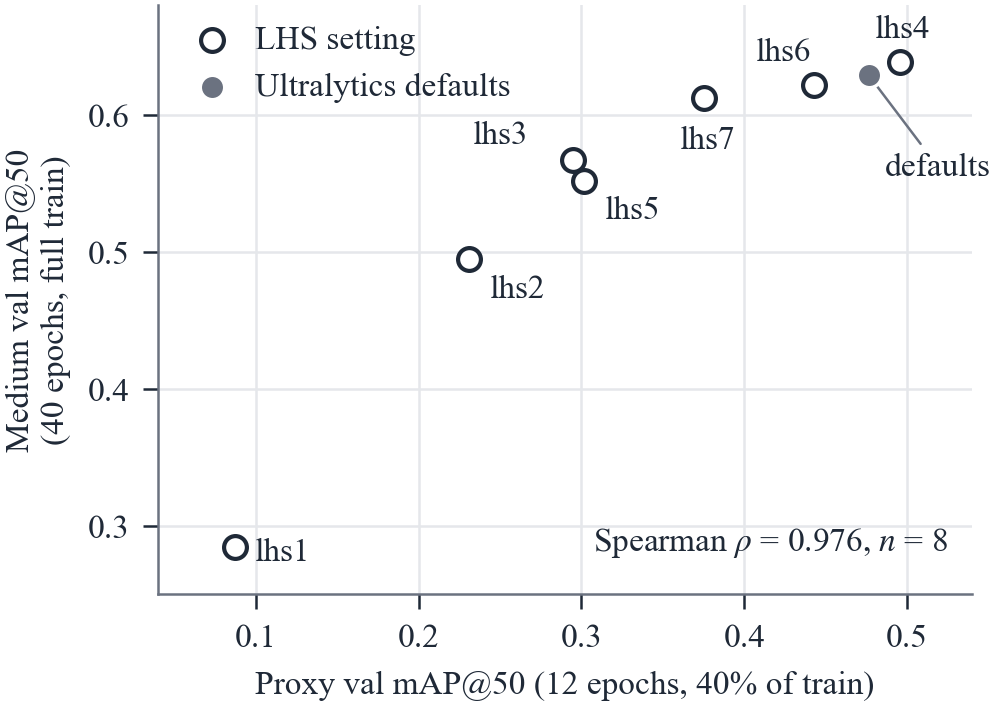
\includegraphics[width=\columnwidth]{r_proxy.png}
\caption{Proxy versus medium validation \mapfifty for the eight settings of the \genone proxy-validity check. The rankings agree except for the adjacent pair lhs3 and lhs5.}
\label{fig:proxy}
\end{figure}

A second, indirect check uses configurations that both generations evaluated. With the same seeds and search space, random search drew the same 32 configurations in both generations. PSO's positions depend on the fitness only through the personal and global bests, which coincided long enough for the swarm to visit identical positions in rounds 1--3 (24 evaluations) but not in round~4. On these repeated configurations, the proxy scores of the two generations have Spearman correlations of 0.991 (random search) and 0.892 (PSO), recomputed from the four search logs. This compares proxy with proxy, not proxy with longer training: the generations order settings alike, but this does not replace a proxy-validity check for \gentwo.

\subsection{Search Behavior}
\label{subsec:res-search}

Fig.~\ref{fig:convergence} shows every proxy evaluation and the best score so far. In \genone, random search found its best setting (0.4995 proxy \mapfifty) at its second evaluation and never improved on it. PSO improved in steps, from 0.4894 after round~1 to 0.4942 after round~3 and 0.4953 in round~4 (evaluation 27), and the swarm converged as intended: the round means rose from 0.393 to 0.423, 0.450 and 0.482, and the within-round standard deviation fell from 0.122 to 0.088, 0.047 and 0.011. The defaults scored 0.4765 on the same proxy, above 28 of the 32 random-search and 21 of the 32 PSO evaluations. The two winners differ by only 0.0042, and lhs4 of the proxy check (0.4955) lies between them. All four search winners of the two generations use a smaller initial learning rate than the default of 0.01 (0.0025 to 0.0070).

\begin{figure*}[!t]
\centering
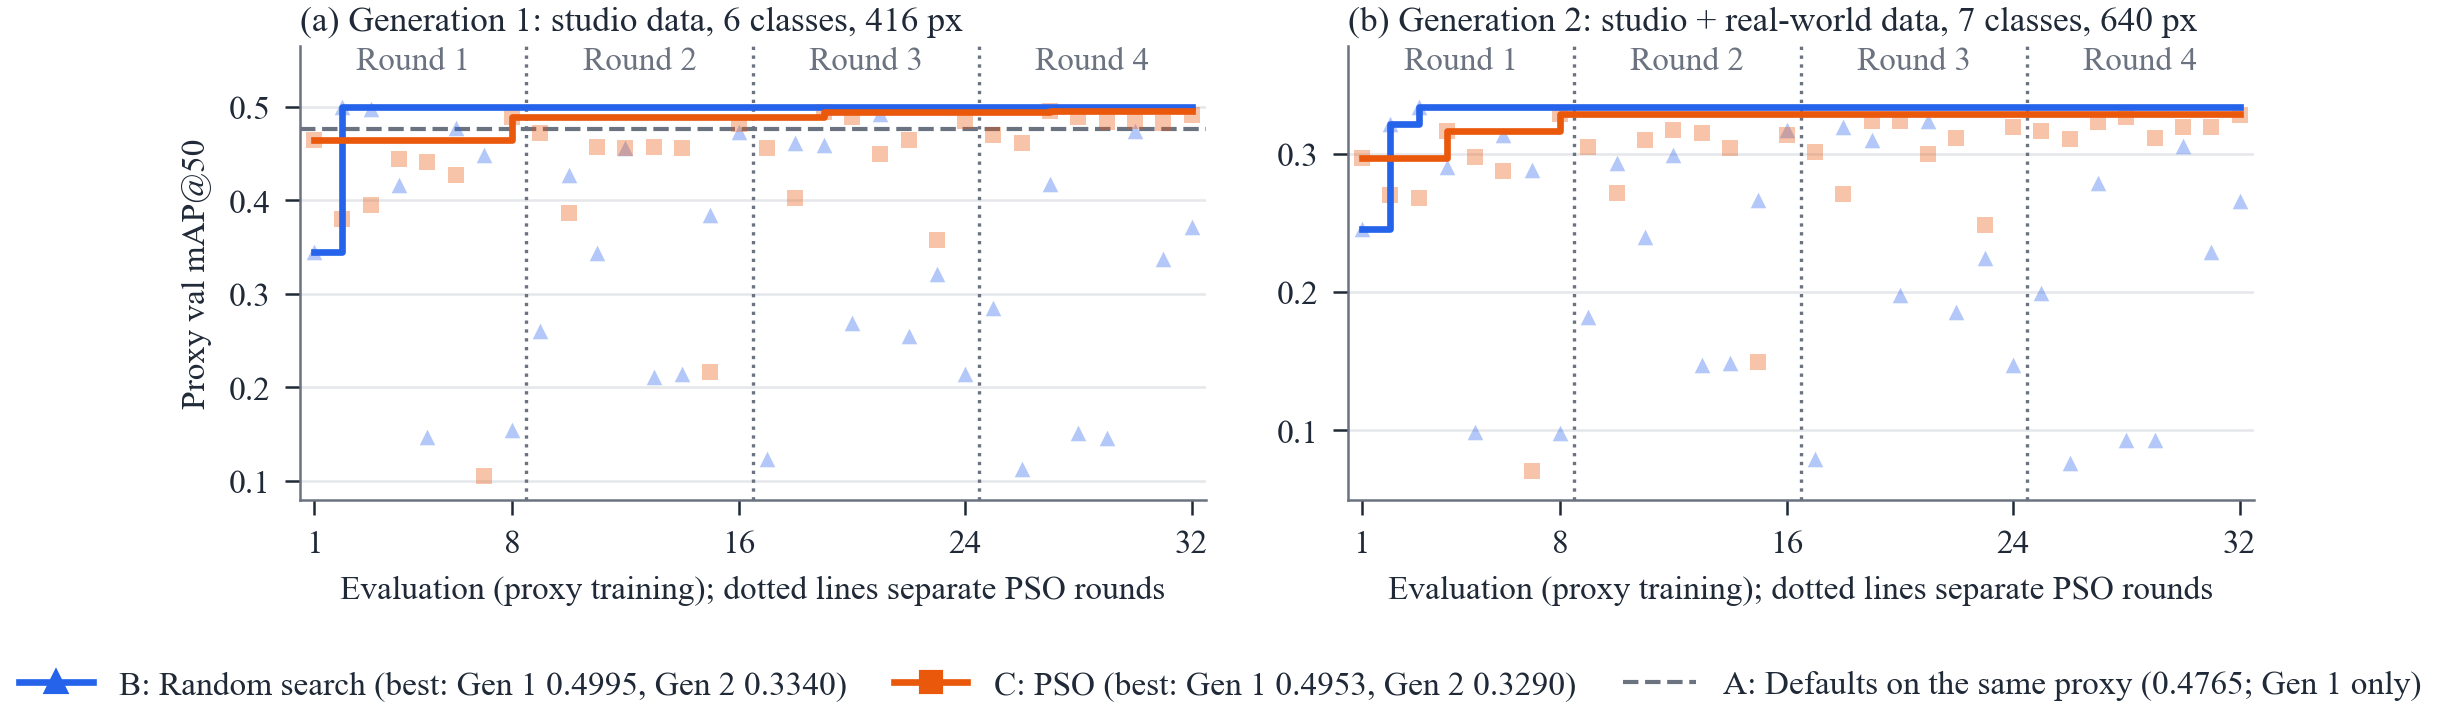
\includegraphics[width=\textwidth]{r_convergence.png}
\caption{Search convergence on the proxy fitness (validation \mapfifty after 12 epochs on 40\% of the training split). Pale markers are individual evaluations (triangles: random search; squares: PSO); solid lines are the best score so far. Dotted lines separate the four PSO rounds of eight particles; random search has no rounds and is plotted in sampling order. The dashed line in (a) is the score of the defaults on the same proxy; \gentwo has no such run. Proxy scores are not comparable between the panels, because the validation sets, classes and image sizes differ.}
\label{fig:convergence}
\end{figure*}

In \gentwo, random search again peaked early (0.3340 at evaluation~3). PSO's best, 0.3290, was the last particle of round~1 and was never beaten (round bests 0.3176, 0.3237 and 0.3279 afterwards), although the swarm still converged: the round means rose from 0.267 to 0.286, 0.300 and 0.319, and the within-round standard deviation fell from 0.082 to 0.006. In both generations, PSO's mean proxy score over all 32 evaluations exceeded that of random search (\genone 0.437 against 0.333; \gentwo 0.293 against 0.226), which reflects the swarm concentrating its later evaluations near good points rather than finding better ones. \gentwo has no proxy run of the defaults, so their standing on the \gentwo proxy is unknown.

\subsection{Generation~1 Test Results (Studio Data)}
\label{subsec:res-gen1}

Table~\ref{tab:gen1-test} gives the one-time test results of the three \genone models on the 1,046 studio test images (7,415 boxes as counted by the evaluator; Table~\ref{tab:datasets} lists 7,413 because it leaves out 2 zero-size boxes). The arms score 0.676 (A), 0.672 (B) and 0.668 (C) \mapfifty, and every pairwise 95\% interval contains 0 on both metrics; the largest difference is C$-$A, $-0.008$ [$-0.021$, $+0.007$]. On studio data, the three arms are therefore statistically tied, and the point estimates even place the defaults first and PSO last; precision and recall are nearly identical. Validation points the same way: the defaults and PSO both reached 0.657, while random search, whose setting had the highest \genone proxy score, reached the lowest value, 0.643.

\begin{table*}[!t]
\centering
\caption{\genone Test Results on the Studio Test Split (1,046 Images)}
\label{tab:gen1-test}
\footnotesize
\begin{tabular}{@{}lcccccc@{}}
\toprule
Arm & Val \mapfifty & Test \mapfifty [95\% CI] & Test \mapfiftyninetyfive [95\% CI] & P & R & ms/img \\
\midrule
A: Defaults & 0.657 & 0.676 [0.639, 0.722] & 0.474 [0.441, 0.518] & 0.747 & 0.581 & 31.4 \\
B: Random search & 0.643 & 0.672 [0.634, 0.717] & 0.475 [0.441, 0.519] & 0.746 & 0.587 & 38.3 \\
C: PSO & 0.657 & 0.668 [0.627, 0.717] & 0.471 [0.437, 0.516] & 0.747 & 0.586 & 31.7 \\
\bottomrule
\end{tabular}
\\[6pt]
\begin{tabular}{@{}lccccc@{}}
\toprule
Pair & $\Delta$\mapfifty [95\% CI] & $P(\Delta>0)$ & $\Delta$\mapfiftyninetyfive [95\% CI] & $P(\Delta>0)$ & Verdict \\
\midrule
B$-$A & $-0.004$ [$-0.016$, $+0.009$] & 0.30 & $+0.001$ [$-0.008$, $+0.010$] & 0.59 & not significant \\
C$-$A & $-0.008$ [$-0.021$, $+0.007$] & 0.16 & $-0.003$ [$-0.012$, $+0.007$] & 0.34 & not significant \\
C$-$B & $-0.004$ [$-0.015$, $+0.007$] & 0.24 & $-0.003$ [$-0.011$, $+0.004$] & 0.19 & not significant \\
\bottomrule
\end{tabular}
\\[2pt]
\parbox{\textwidth}{\footnotesize Val: best checkpoint on the validation split after 100 epochs. CIs: 1,000 paired bootstrap resamples of the test images. P and R at the confidence of maximum F1. ms/img: median batch-1 latency at 416~px on a laptop CPU (Intel Core Ultra~5 125H). $P(\Delta>0)$: share of resamples in which the first arm of the pair scored higher. A difference is significant only if its CI excludes 0.}
\end{table*}

Per class (Fig.~\ref{fig:gen1-perclass}; per-class AP has no confidence interval, Section~\ref{subsec:eval}), the arms differ by less than 0.02 AP@50 on five of the six classes. The exception is PLASTIC, where PSO scores 0.638 against 0.699 (A) and 0.693 (B); PSO is highest on BIODEGRADABLE, GLASS and METAL. The three networks share one architecture, so the higher CPU latency of B (Table~\ref{tab:gen1-test}) most likely reflects other load on the laptop during timing.

\begin{figure}[!t]
\centering
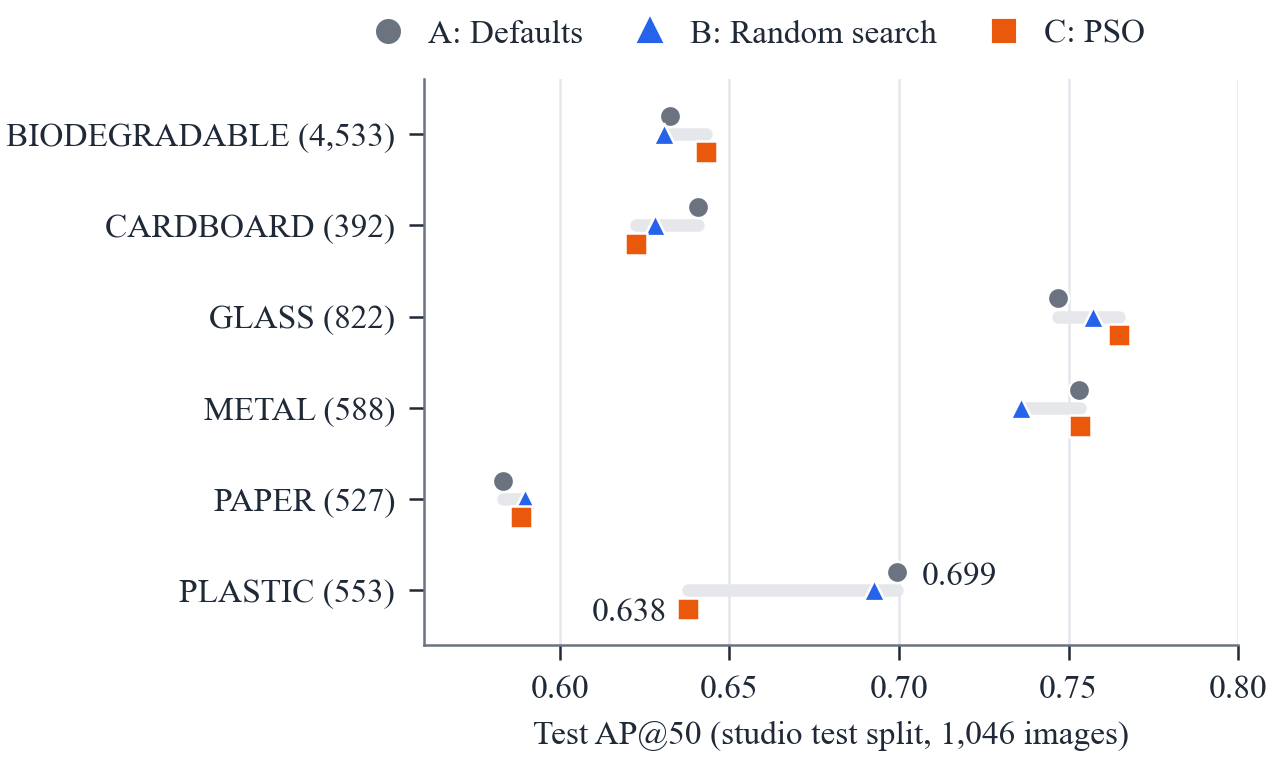
\includegraphics[width=\columnwidth]{r_gen1_per_class.png}
\caption{Per-class test AP@50 of the three \genone models on the studio test split. Numbers in parentheses are the test boxes per class as counted by the evaluator (7,415 in total, including 2 zero-size BIODEGRADABLE boxes); the gray bar spans the three arms' values. PSO is lowest on PLASTIC; elsewhere the arms are within 0.02 of each other.}
\label{fig:gen1-perclass}
\end{figure}

\subsection{Generation~2 Test Results (Mixed Data)}
\label{subsec:res-gen2}

Table~\ref{tab:gen2-test} reports the one-time \gentwo test results on the whole test split and on each domain. On the whole split, the defaults score 0.479, random search 0.497 and PSO 0.500 \mapfifty. Both tuned arms are significantly better than the defaults (B$-$A $+0.017$ [$+0.006$, $+0.030$], C$-$A $+0.020$ [$+0.011$, $+0.032$]), whereas PSO and random search cannot be told apart (C$-$B $+0.003$ [$-0.008$, $+0.015$]). The single-arm intervals overlap widely; the gains are resolved only because the paired bootstrap cancels the variation in image difficulty that all three models share. The \mapfiftyninetyfive verdicts agree with the \mapfifty verdicts everywhere. Random search led PSO on validation (0.473 against 0.466), but on test the two tie.

Studio images contribute 7,413 of the 8,192 boxes, and the studio test set alone (the 1,046 \genone test images) gives the same picture: B$-$A ($+0.024$) and C$-$A ($+0.019$) are significant, C$-$B ($-0.005$) is not. PSO and random search thus differ significantly only on the Indian test set, where all scores are near zero (Section~\ref{subsec:res-domain}).

\begin{table*}[!t]
\centering
\caption{\gentwo Test Results per Test Set: \mapfifty and \mapfiftyninetyfive [95\% CI] per Arm, and Pairwise Differences in \mapfifty}
\label{tab:gen2-test}
\footnotesize
\begin{tabular}{@{}lcccc@{}}
\toprule
 & All & Studio & Real-world & India (DWSD) \\
 & 1,514 img., 8,192 boxes & 1,046 img., 7,413 boxes & 468 img., 779 boxes & 700 img., 4,502 boxes \\
\midrule
\multicolumn{5}{@{}l}{\textit{Test \mapfifty [95\% CI]}} \\
A: Defaults & 0.479 [0.453, 0.513] & 0.571 [0.529, 0.619] & 0.310 [0.278, 0.440] & 0.027 [0.024, 0.031] \\
B: Random search & 0.497 [0.471, 0.531] & 0.595 [0.557, 0.639] & 0.298 [0.271, 0.407] & 0.023 [0.021, 0.027] \\
C: PSO & 0.500 [0.474, 0.534] & 0.590 [0.550, 0.635] & 0.310 [0.279, 0.415] & 0.027 [0.024, 0.031] \\
\midrule
\multicolumn{5}{@{}l}{\textit{$\Delta$\mapfifty [95\% CI] (bold: significant, CI excludes 0)}} \\
B$-$A & $\mathbf{+0.017}$ [$+0.006$, $+0.030$] & $\mathbf{+0.024}$ [$+0.009$, $+0.038$] & $-0.012$ [$-0.118$, $+0.053$] & $\mathbf{-0.003}$ [$-0.006$, $-0.001$] \\
C$-$A & $\mathbf{+0.020}$ [$+0.011$, $+0.032$] & $\mathbf{+0.019}$ [$+0.005$, $+0.033$] & $+0.001$ [$-0.111$, $+0.065$] & $+0.000$ [$-0.003$, $+0.003$] \\
C$-$B & $+0.003$ [$-0.008$, $+0.015$] & $-0.005$ [$-0.018$, $+0.009$] & $+0.013$ [$-0.015$, $+0.036$] & $\mathbf{+0.003}$ [$+0.001$, $+0.006$] \\
\midrule
\multicolumn{5}{@{}l}{\textit{Test \mapfiftyninetyfive [95\% CI]}} \\
A: Defaults & 0.329 [0.309, 0.358] & 0.386 [0.356, 0.425] & 0.254 [0.224, 0.371] & 0.015 [0.013, 0.018] \\
B: Random search & 0.342 [0.322, 0.372] & 0.404 [0.374, 0.442] & 0.238 [0.213, 0.330] & 0.013 [0.012, 0.015] \\
C: PSO & 0.343 [0.323, 0.374] & 0.398 [0.367, 0.439] & 0.248 [0.220, 0.336] & 0.015 [0.013, 0.017] \\
\bottomrule
\end{tabular}
\\[2pt]
\parbox{\textwidth}{\footnotesize All test sets were scored once, at 640~px, with 1,000 paired bootstrap resamples per test set. ``All'' is the whole \gentwo test split (studio plus real-world); India is DWSD, used for testing only. The \mapfiftyninetyfive differences give the same verdict as the \mapfifty differences in every cell. Validation \mapfifty: A 0.454, B 0.473, C 0.466.}
\end{table*}

Per class on the whole split, PSO has the highest AP@50 on five of the seven classes, random search on BIODEGRADABLE and PLASTIC, and the defaults on none. OTHER is very weak for every arm (AP@50 0.050--0.063); all 132 OTHER test boxes are in the real-world images. Precision rises from 0.549 (A) to 0.563 (B) and 0.582 (C), and recall from 0.445 (A) to 0.470 for both tuned arms. The median latency on the T4 at 640~px is 8.1 to 8.7~ms per image.

\subsection{Domain Gap}
\label{subsec:res-domain}

Averaged over the three \gentwo arms, test \mapfifty falls from about 0.59 on studio images to 0.31 on real-world and 0.03 on Indian images (Fig.~\ref{fig:domains}); for every arm, the real-world score is roughly half the studio score.

\begin{figure}[!t]
\centering
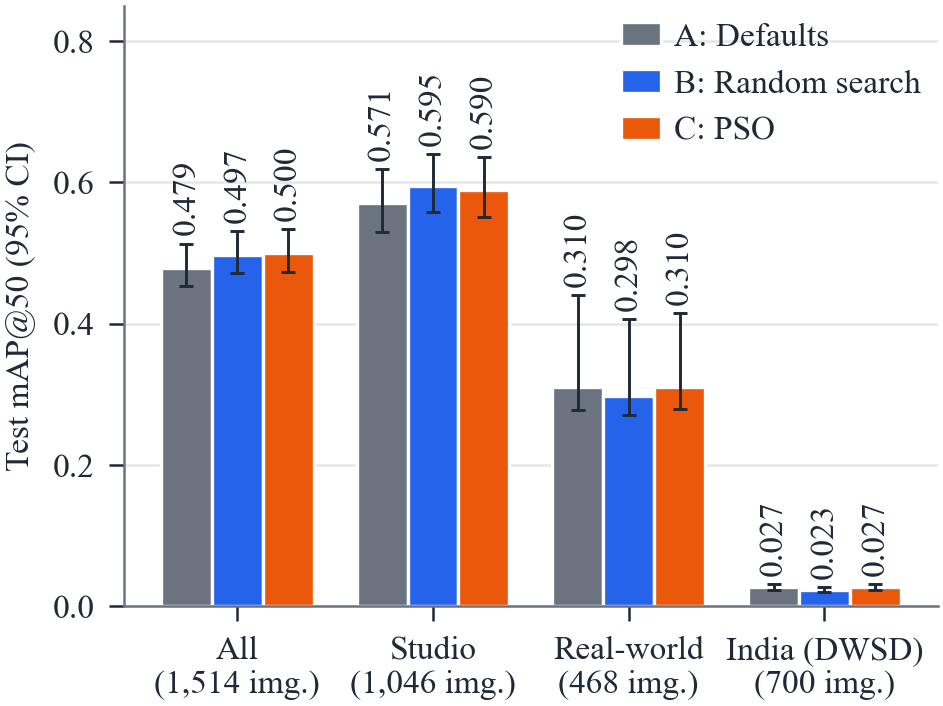
\includegraphics[width=\columnwidth]{r_domains.png}
\caption{Test \mapfifty of the three \gentwo models per test set, with 95\% paired-bootstrap confidence intervals. ``All'' combines the studio and real-world test images; India (DWSD) was used for testing only. The real-world intervals are lopsided because that set holds a single BIODEGRADABLE box.}
\label{fig:domains}
\end{figure}

On the 468 real-world test images (TACO and HITL), no pairwise difference is significant (Table~\ref{tab:gen2-test}). The intervals are wide and lopsided because BIODEGRADABLE has a single box in this set: whether a resample leaves out or repeats that image swings that class's AP, one seventh of the mean, and the arms score 0.249 (A), 0.020 (B) and 0.003 (C) AP@50 on that box. With B$-$A and C$-$A intervals 0.17 to 0.18 wide, this set cannot resolve differences of the size measured on studio images (about 0.02).

On the 700 DWSD images from India, all three models fail, with 0.023 to 0.027 \mapfifty, precision 0.070--0.075 and recall 0.043--0.047; only PLASTIC (0.089--0.101) and PAPER (0.028--0.035) exceed 0.01 AP@50. The defaults and PSO are both significantly above random search and do not differ from each other. On \mapfiftyninetyfive, the two significant differences are B$-$A $-0.002$ [$-0.003$, $-0.001$] and C$-$B $+0.002$ [$+0.000$, $+0.003$], whose lower bound is 0.0004 before rounding. These differences are a few thousandths on scores near zero, so they carry no practical meaning.

Four causes of the failure are known from the data (Section~\ref{subsec:datasets}): no Indian image was used for training, search or model selection; the DWSD images look augmented (rotated, with black corners and color tints), unlike any training image; DWSD's boxes come from mask regions, so touching items of one class merge into one large box that per-item detections overlap poorly, and even correct detections often count as misses; and the mapping from mask values to classes was inferred from the images, with six of the fifteen values uncertain. The India score thus measures the difference in labeling style as well as the models. Fig.~\ref{fig:samples} shows the three models on two studio, two real-world and two DWSD test images. On the two real-world images, which hold eight objects each, every model finds at most three objects of the first and none of the second. On the DWSD images each model predicts at most one box, against 4 and 19 ground-truth boxes, and on the first of them all three models box the region that the ground truth labels PAPER but call it PLASTIC.

\begin{figure*}[p]
\centering
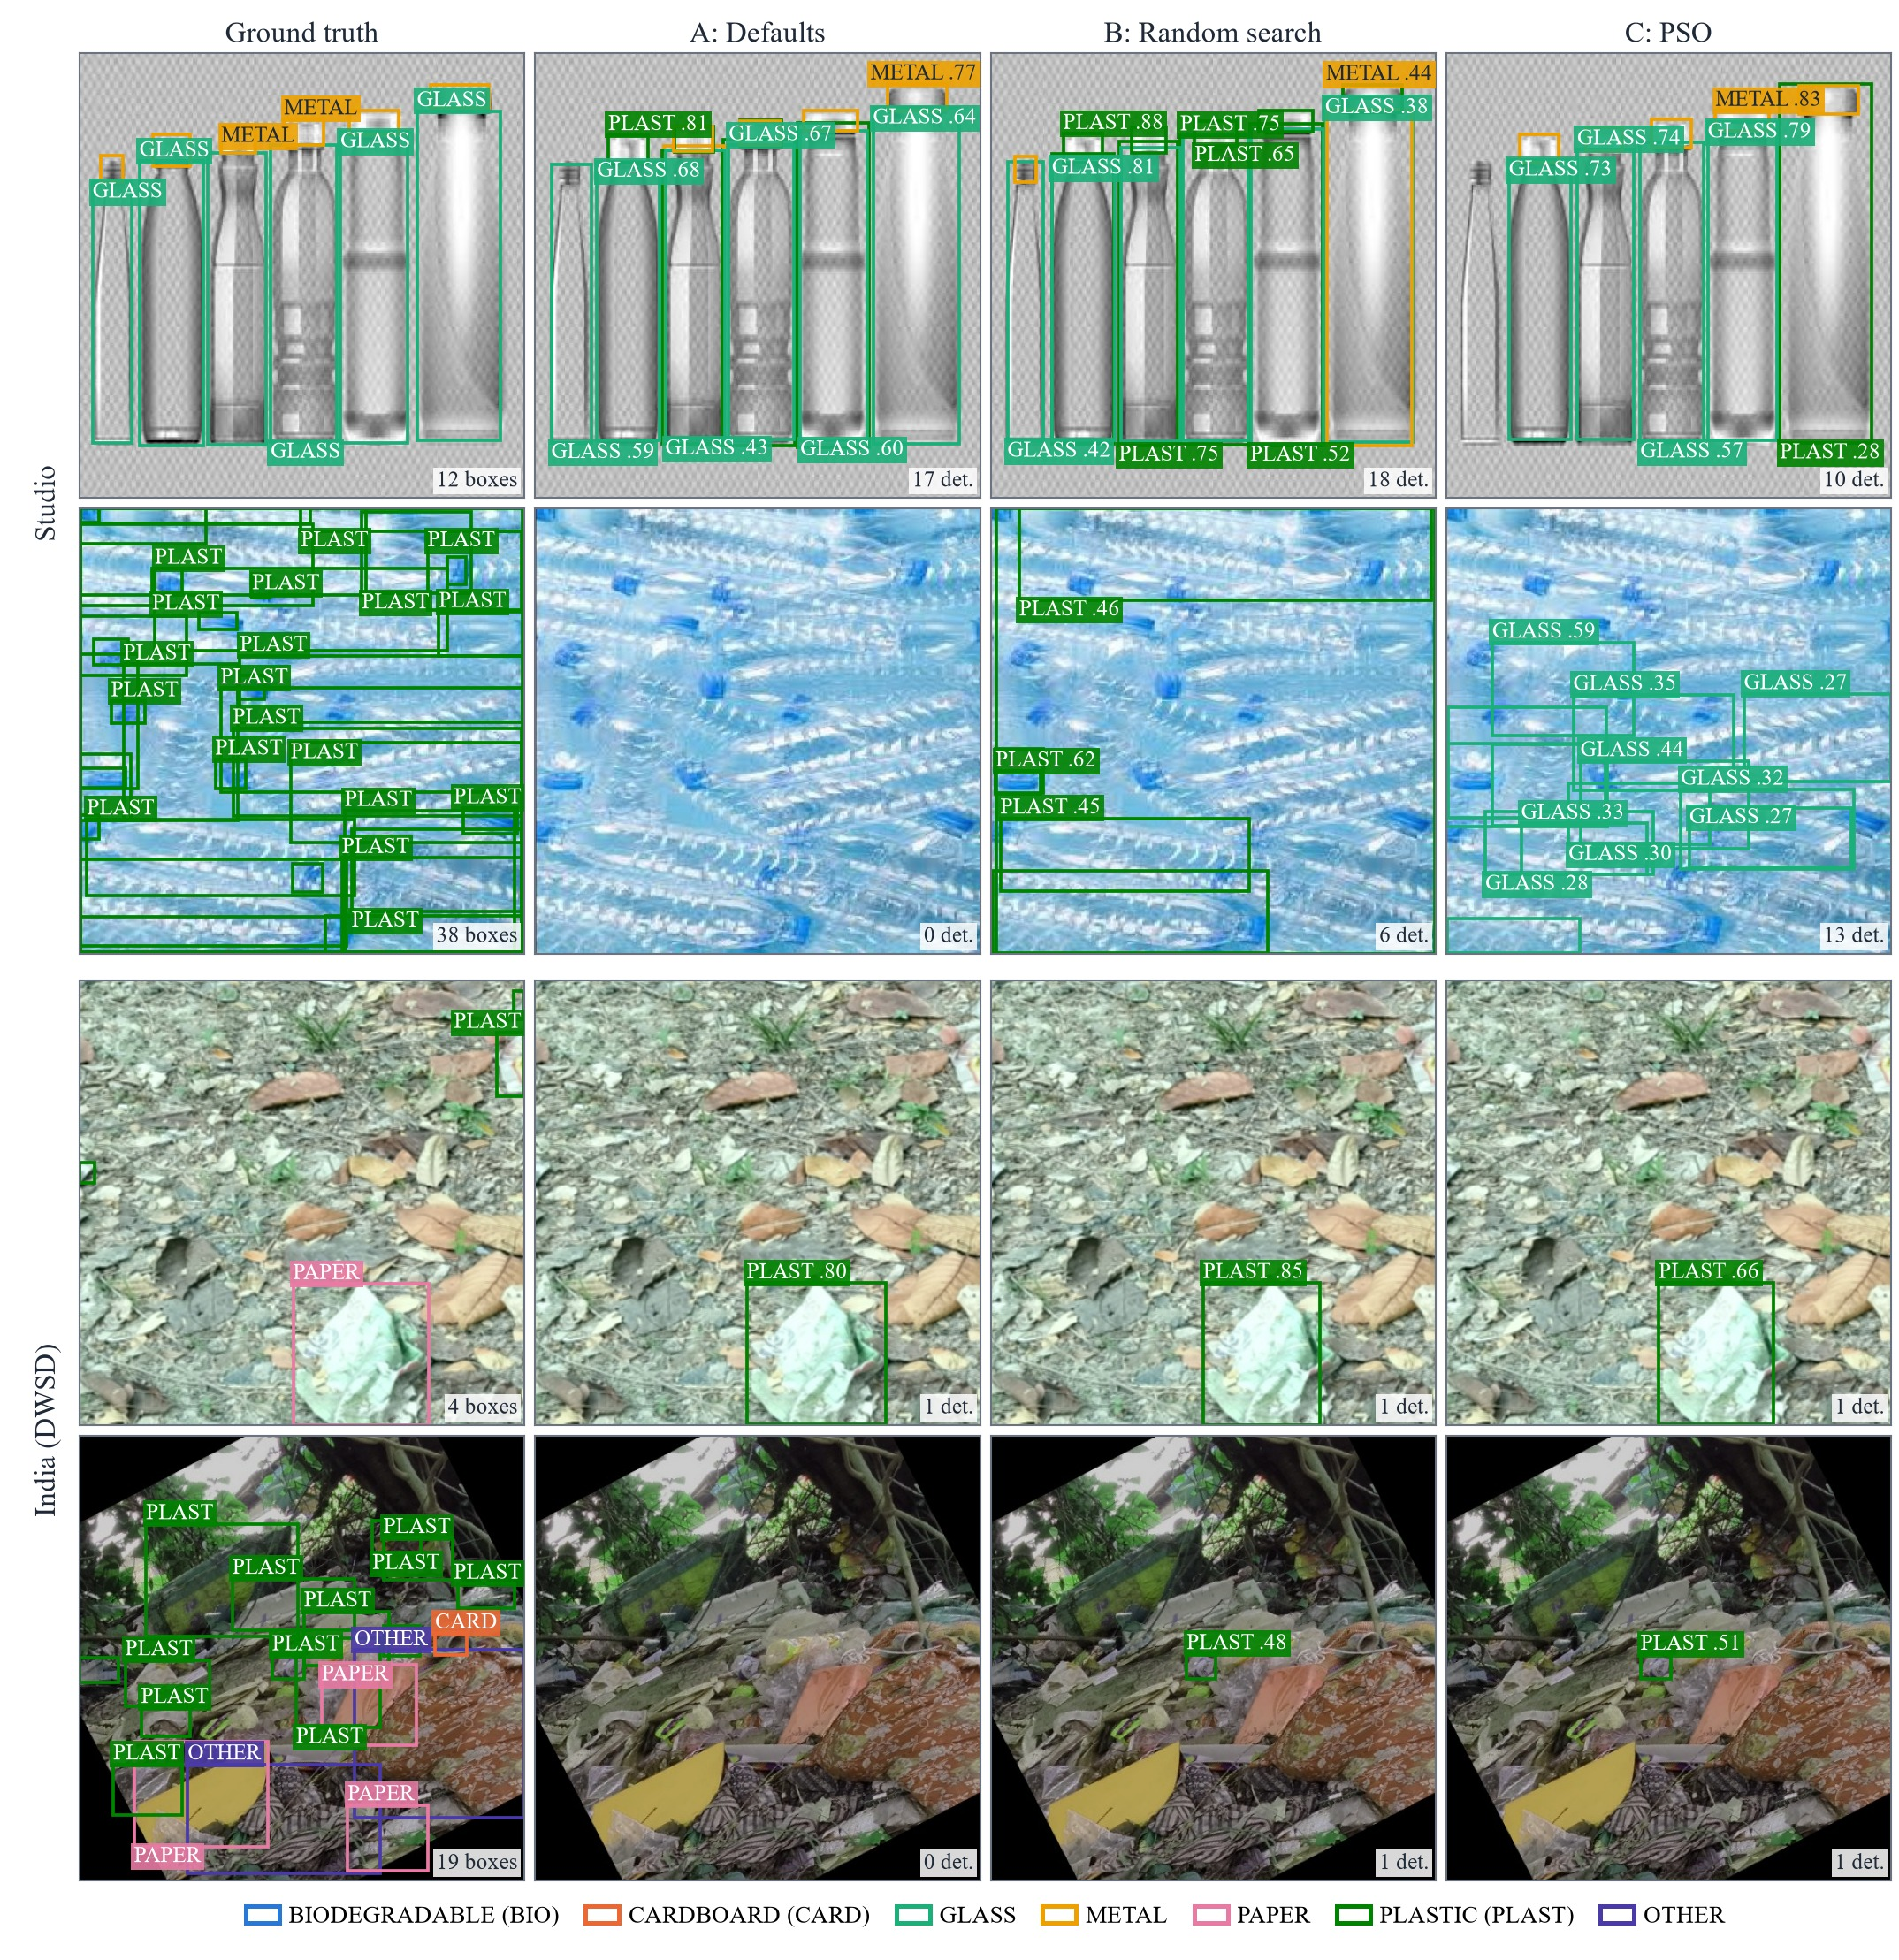
\includegraphics[width=0.85\textwidth]{r_samples.jpg}
\caption{Detections of the three \gentwo models on two studio, two real-world and two Indian (DWSD) test images, next to the ground truth. The images were chosen by a fixed rule, not by eye: for each test set, the images with at least three ground-truth boxes were put in a random order with seed 0, and the first two are shown. Every model saw the same images at 640~px, with a confidence threshold of 0.25 and an NMS IoU of 0.7; the real-world rows show the predictions recorded in the per-image analysis of Fig.~\ref{fig:best}. Each box carries its class and, for predictions, its confidence; a label that would cover another is left out. The corner of each panel gives the number of ground-truth boxes or detections. These panels are illustrations, not evidence; the quantitative results are in Table~\ref{tab:gen2-test} and Fig.~\ref{fig:domains}. The DWSD ground-truth boxes come from mask regions, so touching items of one class can merge into one box.}
\label{fig:samples}
\end{figure*}

The two generations differ in classes, image size and training data, so Tables~\ref{tab:gen1-test} and~\ref{tab:gen2-test} are not one benchmark. Table~\ref{tab:g1g2} therefore scores all six final models on the same studio and real-world test images, restricted to the six shared classes (Section~\ref{subsec:eval}). On the real-world images, every \gentwo arm is significantly better than every \genone arm: 0.338--0.353 \mapfifty against 0.038--0.096, about four to nine times as high. On the studio images, the order reverses: every \genone arm is significantly better than every \gentwo arm, by 0.074 to 0.105. Within each generation, no real-world difference is significant (e.g., \genone C$-$A $+0.048$ [$-0.020$, $+0.163$], \gentwo C$-$B $+0.013$ [$-0.019$, $+0.042$]), and the studio verdicts match Tables~\ref{tab:gen1-test} and~\ref{tab:gen2-test}. The 0.096 of \genone C and its wide interval come largely from the single real-world BIODEGRADABLE box, on which it scores 0.332 AP@50. \gentwo scores higher on real-world images here than in Table~\ref{tab:gen2-test} (A 0.353 against 0.310) only because OTHER is left out of the mean. As a check, \genone reproduces its own studio test result within 0.0004 \mapfifty.

\begin{table}[!t]
\centering
\caption{\genone versus \gentwo on the Same Test Images: Test \mapfifty [95\% CI] on the Six Shared Classes}
\label{tab:g1g2}
\footnotesize
\begin{tabular}{@{}lcc@{}}
\toprule
Model (px) & Real-world (468 img.) & Studio (1,046 img.) \\
\midrule
G1 A (416) & 0.047 [0.038, 0.080] & 0.676 [0.641, 0.719] \\
G1 B (416) & 0.038 [0.031, 0.069] & 0.672 [0.636, 0.716] \\
G1 C (416) & 0.096 [0.041, 0.214] & 0.669 [0.628, 0.716] \\
\midrule
G2 A (640) & 0.353 [0.315, 0.504] & 0.571 [0.529, 0.619] \\
G2 B (640) & 0.338 [0.304, 0.473] & 0.595 [0.557, 0.639] \\
G2 C (640) & 0.352 [0.315, 0.485] & 0.590 [0.550, 0.635] \\
\midrule
$\Delta$ G2$-$G1 & $+0.243$ to $+0.315$ & $-0.105$ to $-0.074$ \\
\bottomrule
\end{tabular}
\\[2pt]
\parbox{\columnwidth}{\footnotesize G1, G2: \genone, \gentwo; each model was scored once at its own training image size (px). Real-world: 647 boxes after removing OTHER, with a single BIODEGRADABLE box; studio: 7,413 boxes, no OTHER. CIs: 1,000 paired bootstrap resamples per test set. $\Delta$: range over all nine G2$-$G1 pairs, every one significant; e.g., real-world G2 B$-$G1 C $+0.243$ [$+0.134$, $+0.418$], studio G2 A$-$G1 A $-0.105$ [$-0.125$, $-0.084$]. On the five real-world classes with more than one box, \gentwo scores 0.239--0.618 AP@50 and \genone 0.008--0.117.}
\end{table}

Where, then, do the \gentwo models succeed on real-world photographs? A per-image analysis of the 468 real-world test images counts an image as fully correct when every ground-truth object is matched by a detection of the same class with IoU $\geq 0.5$ (greedy, highest confidence first, at a confidence threshold of 0.25) and no detection is left unmatched. Each model is fully correct on 166 (A), 168 (B) and 170 (C) images, 35 to 36\% of the set, and all three on the same 111. The successes are almost all single-object photographs: of the 375 images with one object, the models are fully correct on 164 to 167; of the 47 with two objects, on 1 to 4; and of the 46 with three or more, on none. Fig.~\ref{fig:best} shows the most favorable cases, chosen by a fixed rule. No image with three or more objects, and only one with two, is fully correct for all three models, so the rule fell back to the two images with at least two objects that at least two models label fully correctly; one of them is a close-up on a plain background, close to studio conditions. The models thus handle an isolated item in a real scene, but not a cluttered scene with several items.

\begin{figure*}[!t]
\centering
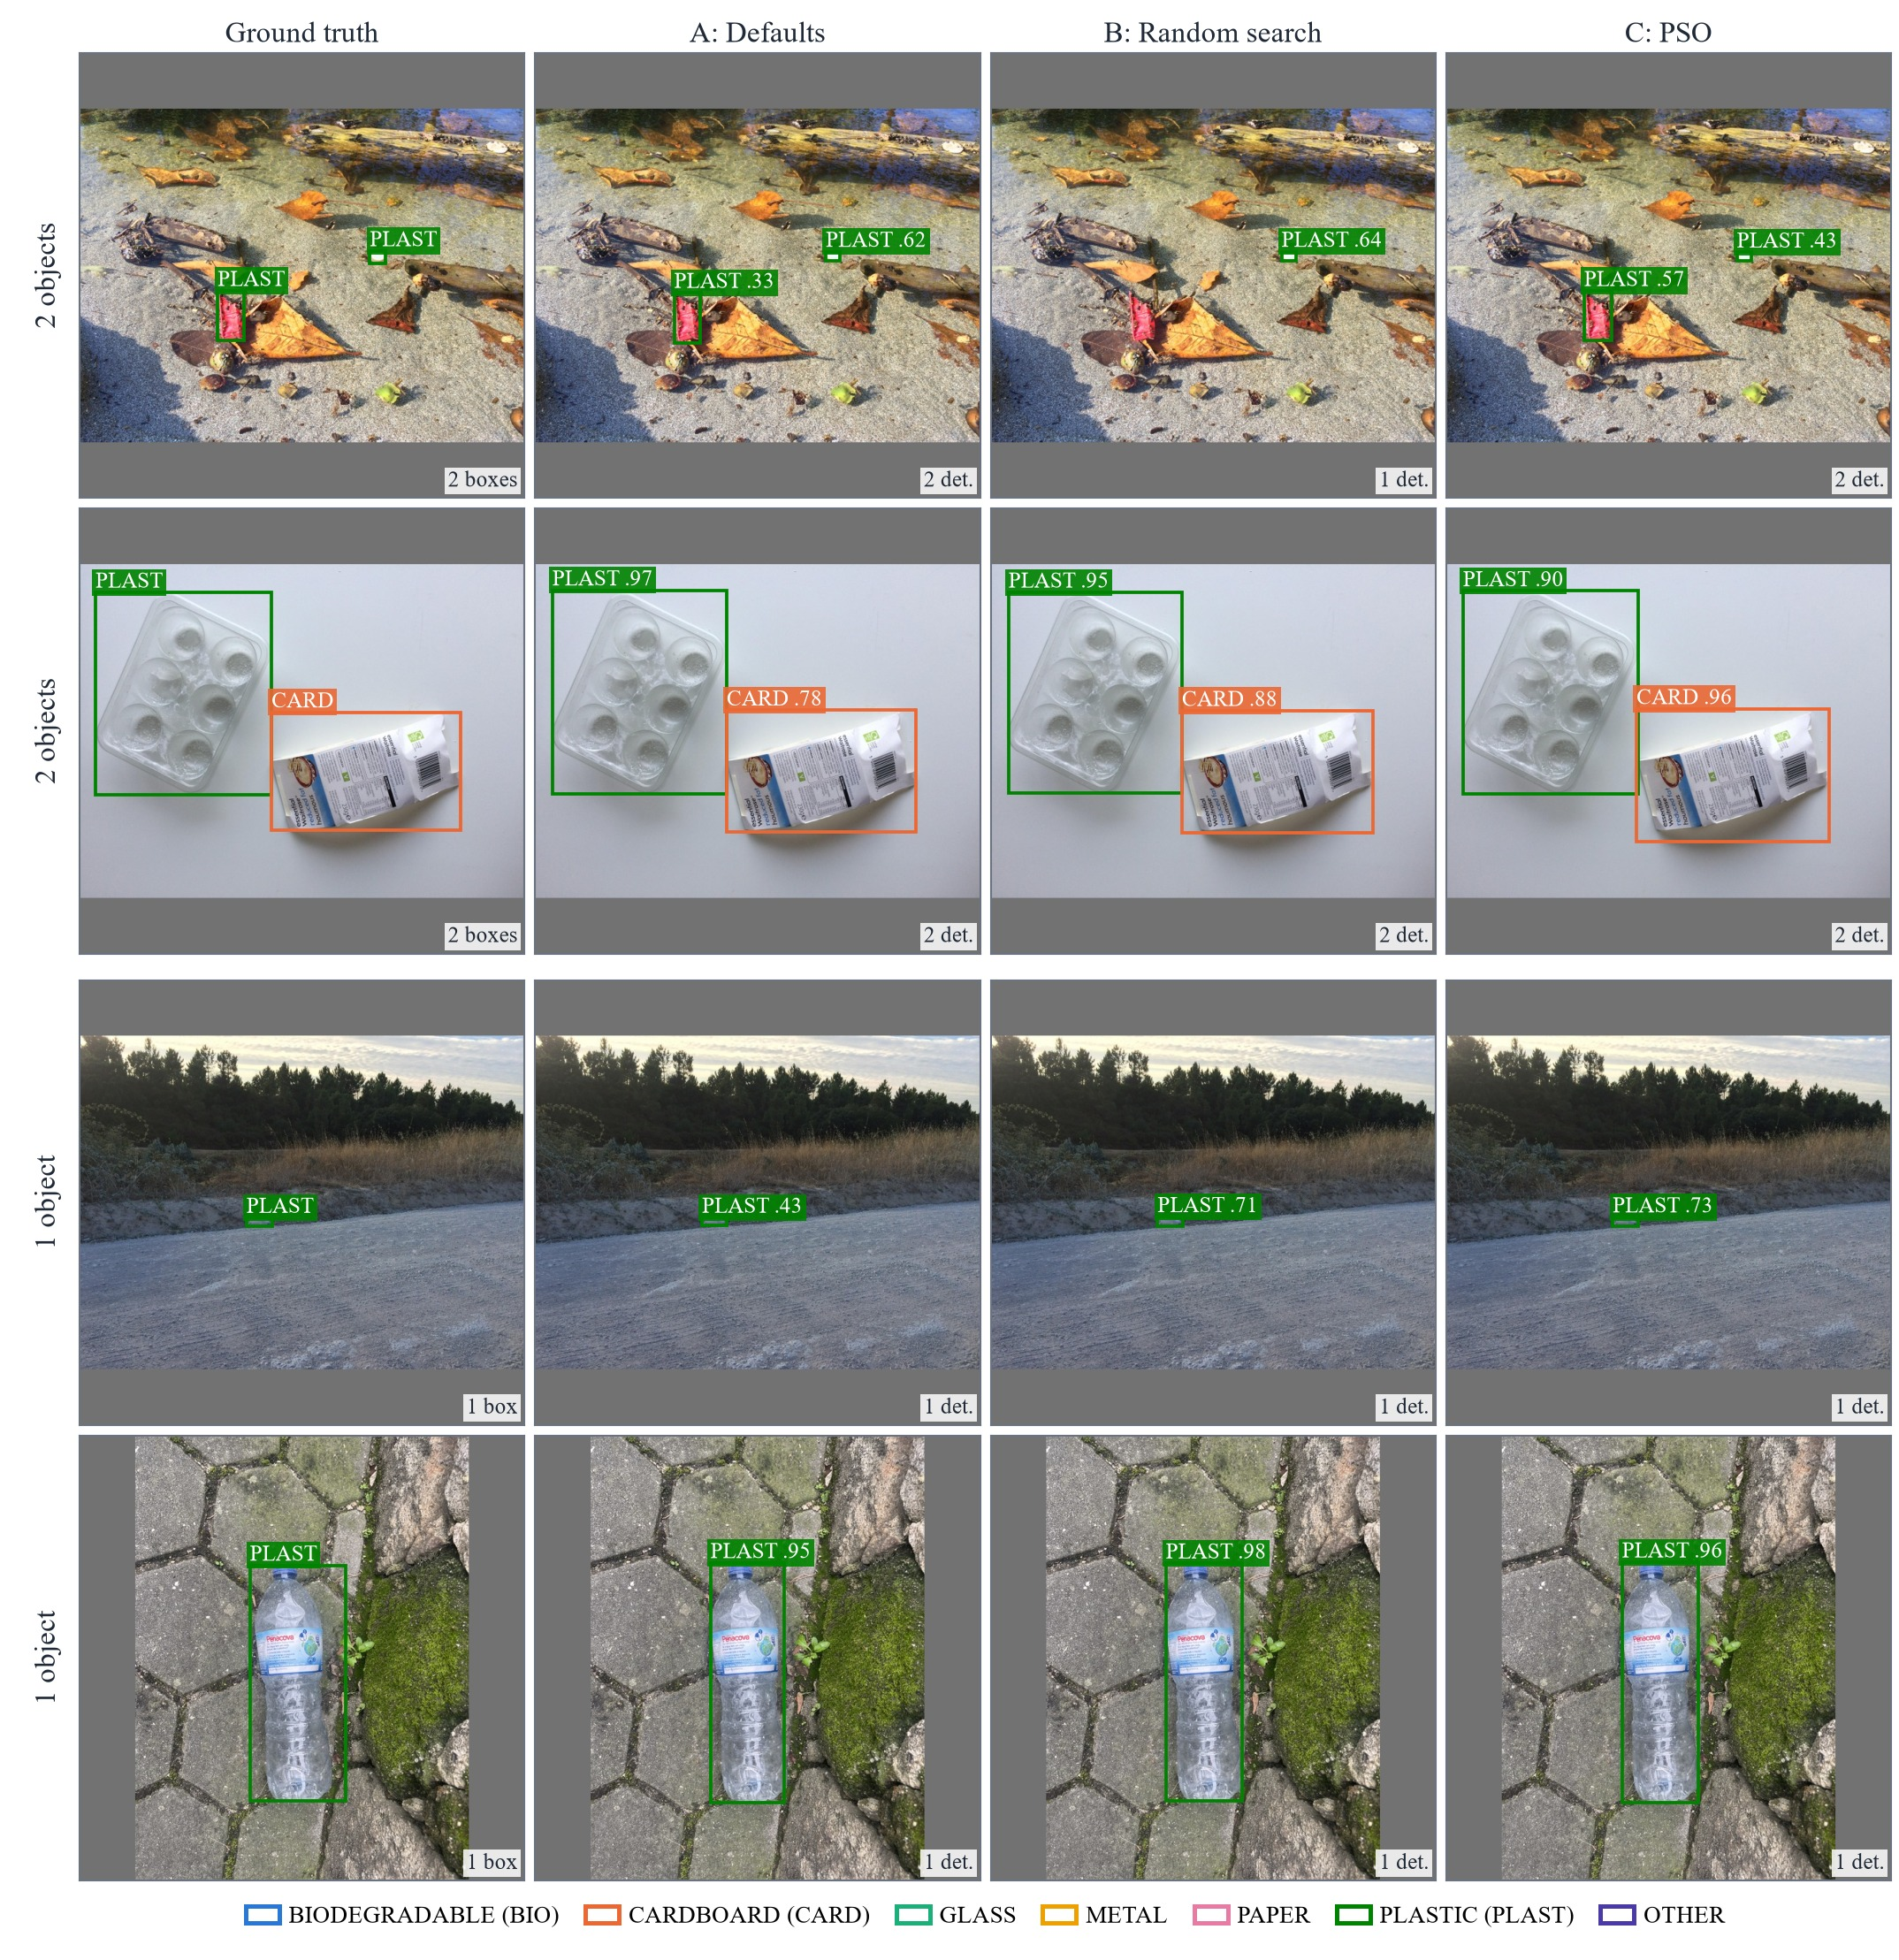
\includegraphics[width=0.8\textwidth]{r_best.jpg}
\caption{Selected success cases on real-world test images: deliberately favorable, not representative. Rows 1--2: the only real-world test images with at least two objects that at least two of the three \gentwo models label fully correctly (every object found with the right class, no false detection); no image with three or more objects qualifies, and random search (B) misses one object in the first. Rows 3--4: the first two of the 110 single-object images that all three models label fully correctly, in a random order with seed 0. Confidence threshold 0.25, NMS IoU 0.7, 640~px. For scale, each model is fully correct on 166--170 of the 468 real-world test images, on 164--167 of the 375 single-object images and on none of the 46 images with three or more objects.}
\label{fig:best}
\end{figure*}

\subsection{Compute Cost}
\label{subsec:res-cost}

Table~\ref{tab:compute} lists the recorded GPU time of every run on one Tesla T4, covering training only (setup, data copies and idle time are excluded). Including its search, each tuned arm cost about 2.7 to 2.8 times the GPU time of Arm~A, which needs no search. The budget was equal in evaluations, not in time: the mean proxy training took 214.3~s for PSO and 238.7~s for random search in \genone, and 285.5~s and 259.0~s in \gentwo. The largest \genone item was the proxy-validity check, of which the eight 40-epoch medium runs took 3.84 of 4.36 hours. In \gentwo, about 24 further GPU-hours were lost when two sessions froze and sat idle until the platform's 12-hour limit; they are not in the totals. The one-time test evaluation took 283.1~s on the laptop CPU in \genone and 220.6~s on the T4 for the four \gentwo test sets.

\begin{table}[!t]
\centering
\caption{Recorded GPU Time per Run (Hours, One Tesla T4)}
\label{tab:compute}
\footnotesize
\begin{tabular}{@{}lcc@{}}
\toprule
Run & \genone & \gentwo \\
\midrule
Proxy-validity check (16 runs) & 4.36 & not run \\
PSO search (32 proxy trainings) & 1.91 & 2.54 \\
Random search (32 proxy trainings) & 2.12 & 2.30 \\
Arm~A full training (100 epochs) & 1.18 & 1.56 \\
Arm~B full training (100 epochs) & 1.15 & 2.07 \\
Arm~C full training (100 epochs) & 1.45 & 1.60 \\
\midrule
Total recorded & 12.18 & 10.06 \\
\bottomrule
\end{tabular}
\\[2pt]
\parbox{\columnwidth}{\footnotesize Sums of the recorded training wall-clock times. The \gentwo random search and Arm~C training were resumed after a session froze (Arm~C after epoch 55); their idle time, about 24 GPU-hours in total, is not included.}
\end{table}

\section{Discussion}
\label{sec:discussion}

This section explains the results (Section~\ref{subsec:why}), draws a recommendation for tuning studies (Section~\ref{subsec:implications}), considers deployment (Section~\ref{subsec:deployment}) and states the limits of the evidence (Section~\ref{subsec:limitations}).

\subsection{Why PSO Did Not Beat Random Search}
\label{subsec:why}

In \genone, the defaults left little room for any search. On the proxy they scored 0.4765 \mapfifty, above 28 of the 32 random-search evaluations and 21 of the 32 PSO evaluations (Section~\ref{subsec:res-search}), and in the proxy-validity check they ranked second of eight on both the proxy and the 40-epoch runs (Table~\ref{tab:proxy}). The best settings of the two searches exceeded them on the proxy by only 0.019 (PSO, 0.4953) and 0.023 (random search, 0.4995), and the four best settings of the check lie within 0.026 of each other after 40 epochs. This suggests a broad, flat region of good settings around the defaults.

Within that region, the proxy could not pick a winner. It separated poor settings from good ones ($\rho = 0.976$), but the gaps among its best candidates did not survive full training: random search's setting, the \genone proxy winner, gave the lowest \genone validation score after 100 epochs (0.643, against 0.657 for the defaults and PSO). A 12-epoch run on 40\% of the data may favor settings that learn quickly, and picking the maximum of 32 single-run scores favors scores that were high by chance; we measured neither effect.

The budget was also small: 32 evaluations in six dimensions, of which PSO spends eight on its random initial swarm and the rest in three update steps. Bergstra and Bengio~\cite{bergstra2012random} report that for most data sets only a few hyperparameters really matter, and that random search finds models as good as or better than grid search at the same budget. If only one or two of our six dimensions matter, 32 independent samples already cover them densely, leaving a guided search little to exploit. All four search winners chose an initial learning rate below the default (0.0025 to 0.0070), which fits this view, although we did not measure the importance of each dimension.

The swarm behaved as designed but converged early. In \genone, the standard deviation of its proxy scores within a round fell from 0.122 to 0.011, and its mean over all 32 evaluations exceeded that of random search (0.437 against 0.333), yet its best setting was not better. In \gentwo, PSO's best setting was the last particle of the random initial swarm, and rounds 2 to 4 never beat it (Fig.~\ref{fig:convergence}), so its chosen setting was in effect the best of eight random samples, competing with the best of 32. A global-best swarm with three update steps concentrates its later evaluations around the best point of round~1; this raises the average evaluation but not the maximum, and only the maximum is used.

Why tuning helped in \gentwo but not in \genone is less clear. Our hypothesis is that the new data, real-world photographs at 640~px with a seventh class, moved the region of good settings away from the defaults, so that any reasonable search gained about 0.02 \mapfifty on the mixed and studio test sets. It cannot be tested with the present runs, because \gentwo has no proxy run of the defaults. An alternative is training noise: with one training seed per arm, the intervals cover test sampling only (Section~\ref{subsec:limitations}), so part of a 0.02 gain could come from the particular training run. Repeating the proxy check and the full trainings for \gentwo would separate the two explanations (Section~\ref{subsec:fw-opt}).

\subsection{Implications for Tuning Claims in Waste AI}
\label{subsec:implications}

Gap~3 (Section~\ref{subsec:gaps}) states that metaheuristic tuning in this area is compared with other metaheuristics or with nothing, and that test results are reported as single numbers. Our results show what such designs can miss. Had \gentwo compared PSO only with the defaults, it would have reported a significant gain of $+0.020$ [$+0.011$, $+0.032$] \mapfifty and credited it to the swarm. Random search, at the same 32 evaluations, gained $+0.017$ [$+0.006$, $+0.030$], and the two tuned arms cannot be told apart, so the gain belongs to searching at all, not to the swarm's guidance. Single numbers would also have misled: the \genone point estimates rank the defaults first and PSO last (0.676, 0.672 and 0.668), and \gentwo validation ranked random search ahead of PSO, yet neither ordering is significant on test. Conversely, PSO's significant $+0.003$ over random search on India shows that an interval excluding zero is not enough: on scores near 0.02, such a difference has no practical meaning.

We therefore recommend a minimum protocol for any claim that a metaheuristic tunes a waste model better. First, include the defaults and random search as arms at the same number of evaluations, and report the time spent, since equal evaluations need not mean equal time (Section~\ref{subsec:res-cost}). Second, if a cheap proxy is used, check before the search that it ranks settings like longer training, against a threshold fixed in advance. Third, choose each arm's final setting on validation data and score the test split once. Fourth, report paired confidence intervals on the differences between arms, per test domain, and judge them against a difference that would matter in use. Fifth, repeat trainings and searches with several seeds. SwarmSort meets the first four points but not the fifth. In an equal-budget comparison such as that of Sayed et al.~\cite{sayed2024intelligent}, a random-search arm would cost no more than one further competitor.

\subsection{Real-World and Indian Deployment}
\label{subsec:deployment}

For a smart bin or a municipal service, the domain matters far more than the optimizer. For every arm, the real-world score is roughly half the studio score (0.298--0.310 against 0.571--0.595), and on the Indian photographs all arms collapse to 0.023--0.027 \mapfifty (Section~\ref{subsec:res-domain}). The largest tuning effect we measured, about 0.02, is more than ten times smaller than the studio-to-real-world drop of about 0.28, and it did not appear on real-world photographs at all. Local training data will therefore help more than a better search, which is why Indian data lead the roadmap (Section~\ref{subsec:fw-data}). Whether the real-world training data of \gentwo improved real-world accuracy over \genone is answered by a separate comparison on the same images: \textbf{[PENDING: Gen~1 vs Gen~2 comparison]}.

The India score must be read with its labels in mind. DWSD's boxes come from mask regions in which touching items of one class merge, and its class mapping was inferred from the masks (Section~\ref{subsec:datasets}). A model that correctly finds each bag in a pile overlaps the merged box poorly and is counted wrong, so the score measures the difference in labeling style as well as the model, in unknown proportions. A test set must be labeled like the training data before its score can be read as accuracy; relabeling part of DWSD item by item would separate the two effects.

Deployment in India also constrains the output classes. Rule~15(h) of the Solid Waste Management Rules, 2016~\cite{moefcc2016solid} requires green bins for bio-degradable waste, white bins for recyclable waste and black bins for other waste. BIODEGRADABLE maps to the green bin and the five material classes, insofar as their items are recyclable, to the white bin, but the black bin corresponds to OTHER, the weakest class of every arm (AP@50 0.050 to 0.063). A bin built on these models would be least reliable for exactly the items that belong in the black bin.

\subsection{Limitations and Threats to Validity}
\label{subsec:limitations}

Each arm was trained once (seed 42) and each search was run once (PSO seed 42, random-search seed 123), so the confidence intervals cover the sampling of test images only, not the randomness of training or search, and another seed could change the small differences between arms. No $p$-values or multiple-comparison corrections were computed for the twelve pairwise comparisons per metric in \gentwo (three pairs on four test sets), and per-class AP has no interval. The real-world test set holds a single BIODEGRADABLE box, which makes its intervals wide and lopsided.

The proxy check used eight settings, was run for \genone only, and used a 40-epoch reference rather than the 100 epochs of the final trainings; proxy validity in \gentwo, with new data, classes and image size, is assumed. The proxy also scored last-epoch weights, whereas the final models were selected as the best validation checkpoint (\texttt{best.pt}). The \gentwo Arm~C training was resumed after epoch 55 when a session froze; it continued the same weights and optimizer state but is not bit-identical to an uninterrupted run.

For DWSD, the class mapping was inferred from the masks, with six of the fifteen mask values uncertain, and the boxes come from connected regions rather than single items. Only six training hyperparameters were searched, and the budget was equal in evaluations, not in time. No external baseline was run: we did not reproduce the pipeline of Majchrowska et al.~\cite{majchrowska2022deep} or any other published detector on our data, so our scores cannot be ranked against prior work. Finally, the literature review was targeted rather than systematic (Section~\ref{subsec:review-method}), so the gaps of Section~\ref{subsec:gaps} hold for the literature we reviewed.

\section{Future Work: Possible Improvements}
\label{sec:future}

Each improvement answers a limitation (Section~\ref{subsec:limitations}) or a measured result; Table~\ref{tab:roadmap} orders them by expected value for effort.

\subsection{The Optimization Study}
\label{subsec:fw-opt}

Three training seeds per arm would let the intervals cover training noise, and several search seeds per method would show whether PSO's result repeats. Because the small proxy gaps among the top settings vanished after full training, multi-fidelity search such as successive halving or Hyperband~\cite{li2018hyperband} should promote the best candidates to longer runs before a winner is chosen. Because the swarm converged early (in \gentwo it never improved after round~1), PSO variants could keep it exploring: the constriction factor of Clerc and Kennedy~\cite{clerc2002particle}, a ring topology, adaptive inertia, or more particles and rounds.

Other optimizers should join as further arms against the same baselines at 32 evaluations: a genetic or evolutionary algorithm~\cite{young2015optimizing}, differential evolution~\cite{storn1997differential} and Bayesian optimization such as Optuna's tree-structured Parzen estimator~\cite{akiba2019optuna}. This also answers why PSO and not, say, the beluga whale optimizer of Sayed et al.~\cite{sayed2024intelligent}: the protocol is optimizer-agnostic, and its value is that every candidate meets the same baselines. A wider search space (color augmentation, translation, loss gains, image size) would test whether six settings left too little room to beat the defaults, and a domain-aware fitness scored on real-world validation images targets tuning gains that did not reach real-world photographs. Finally, the proxy check should be repeated for \gentwo against a 100-epoch reference, with a defaults run testing the hypothesis of Section~\ref{subsec:why}, and the statistics strengthened with Holm's correction, per-class AP intervals and stored bootstrap resamples.

\subsection{Data and the Indian Domain}
\label{subsec:fw-data}

The main next step is Indian training data with per-item boxes (part of DWSD or a new collection, with a held-out test part), which addresses the DWSD failure and the labeling mismatch behind part of it; since \gentwo's real-world data cost studio accuracy (Section~\ref{subsec:deployment}), it should be added by domain-aware training, for example keeping all studio images or using a larger model. The weak OTHER class needs more examples, a split into clearer classes, or a merge into existing ones. Clutter augmentations such as copy-paste~\cite{ghiasi2021simple}, smaller object scales, blur and lighting changes target the small, overlapping and partly hidden items of real-world photographs. Finally, the classes could follow the three streams that the SWM Rules 2016 require, bio-degradable, non-bio-degradable and domestic hazardous~\cite{moefcc2016solid}, so that each detection maps to a bin.

\subsection{The Model}
\label{subsec:fw-model}

Larger or newer detectors (YOLOv8s, YOLOv8m, YOLO11~\cite{jocher2024yolo11}) with the same settings would show how much of the real-world gap is due to model capacity, at a cost in speed on edge devices. Sliced inference~\cite{akyon2022slicing} on overlapping tiles suits wide photographs with many small items, and confidence calibration such as temperature scaling~\cite{guo2017calibration} would make a score of 0.5 mean roughly 50\% correct, which matters when a bin acts on a threshold.

\subsection{Combining the Three Models}
\label{subsec:fw-ensemble}

On point estimates, no arm leads on every \gentwo test set (Table~\ref{tab:gen2-test}). On real-world photographs, where the three \mapfifty values lie within 0.012, the arms differ more in their parts: precision at the maximum-F1 confidence ranges from 0.366 (B) to 0.556 (C), PAPER AP@50 from 0.239 (A) to 0.330 (C), and random search leads on GLASS (0.296). These values lack intervals and model agreement was not measured, but they suggest partly different mistakes, so combining the arms, with no extra training, could beat each one alone.

Three combinations should be compared: box fusion, which pools the boxes of A, B and C and merges overlapping ones by weighted boxes fusion~\cite{solovyev2021weighted} or non-maximum suppression; majority voting, which keeps a box only if at least two models find it (IoU $\ge 0.5$) to raise precision and can flag single-model boxes as uncertain instead of discarding them; and weighted voting by each model's validation \mapfifty, never by test scores, which would leak the test split. As a soft-computing extension, a search yields a population of good settings (the final swarm and the best random samples), so training and combining the top-$k$ uses the swarm as an ensemble generator; since the converged swarm may lack diversity, top random samples should be mixed in. Each ensemble should be compared with the best single arm, chosen on validation, by the same paired bootstrap on every test set. Its cost is inference time: about three times as long, roughly 100~ms per image on the laptop CPU against 31 to 38~ms for one \genone model.

\subsection{Deployment}
\label{subsec:fw-deploy}

Per-class confidence thresholds chosen on validation data could replace the single threshold, since real-world precision is low and AP varies widely by class. Because our latencies come only from a laptop CPU and a cloud GPU, the models should be exported to ONNX or TFLite and timed on a Raspberry Pi, the class of hardware Alshammari et al.~\cite{alshammari2025smart} use for a smart-bin classifier, and, since real sorting is continuous, tested on live video.

\begin{table}[!t]
\centering
\caption{Future-Work Roadmap, Ordered by Expected Value for Effort}
\label{tab:roadmap}
\footnotesize
\setlength{\tabcolsep}{3pt}
\renewcommand{\arraystretch}{1.1}
\begin{tabular}{@{}c>{\raggedright\arraybackslash}p{2.75cm}>{\raggedright\arraybackslash}p{3.05cm}>{\raggedright\arraybackslash}p{1.45cm}@{}}
\toprule
Priority & Improvement & Addresses & Effort \\
\midrule
1 & Indian training data with per-item boxes & DWSD failure (0.023--0.027 \mapfifty) & Large \\
2 & Ensemble of A, B and C (fusion or voting) & Arms differ per class and test set; no arm wins everywhere & Small (no training) \\
3 & Three training seeds per arm, several search seeds & Tuning effect vs.\ training noise & Medium \\
4 & Domain-aware fitness (real-world validation) & Tuning gains did not carry to real-world photos & Medium \\
5 & Multi-fidelity search (Hyperband) & Proxy gaps vanish at 100 epochs & Medium \\
6 & GA, DE and Bayesian optimization at the same budget & ``Why PSO?'' & Medium \\
7 & Fix the OTHER class & AP@50 0.050--0.063 & Medium \\
8 & Larger detector; sliced inference & Small items, look-alike materials & Medium \\
9 & Edge export and latency on a Raspberry Pi & Real smart-bin hardware & Medium \\
10 & Swarm as an ensemble generator (top-$k$ settings) & Uses the whole PSO population & Medium \\
\bottomrule
\end{tabular}
\\[2pt]
\parbox{\columnwidth}{\footnotesize Effort: Small = hours, no GPU training; Medium = about a day with some GPU time; Large = several days or a new data pipeline. GA = genetic algorithm; DE = differential evolution.}
\end{table}

\section{Conclusion}
\label{sec:conclusion}

SwarmSort tested whether a particle swarm tunes a lightweight waste detector better than random search or the default settings when all three receive the same budget, and whether the answer holds when the photographs move from the studio to real-world and Indian scenes.

RQ1 asked whether PSO, at an equal budget of 32 proxy trainings, beats random search and the defaults on a held-out test set. It never meaningfully beat random search. In \genone, on studio data, the three arms tied at 0.676, 0.672 and 0.668 \mapfifty, with every interval of the differences containing 0. In \gentwo, both tuned arms beat the defaults on the mixed test set (random search by $+0.017$, PSO by $+0.020$), but PSO and random search could not be told apart on the mixed, studio and real-world test sets; their only significant difference, $+0.003$ on India, lies on scores near 0.02 and has no practical meaning. RQ2 asked whether the short proxy ranks settings like longer training. It did ($\rho = 0.976$, $n = 8$, \genone only), but it could not separate the best settings, whose small proxy gaps vanished after full training. RQ3 asked whether the answer changes with the domain. It does: the tuning gains did not reach real-world photographs (0.298 to 0.310, no significant difference), every arm's real-world score was roughly half its studio score, and all arms failed on the Indian DWSD photographs (0.023 to 0.027), a failure that partly reflects DWSD's merged, mask-derived boxes.

Two messages follow. First, a claim that a metaheuristic tunes a model better needs the defaults and random search at an equal budget, and confidence intervals on a test split used once; without the random-search arm, our \gentwo gain for PSO would have been credited to the swarm. Second, for waste detection in real and especially Indian scenes, local training data matter more than the choice of optimizer. Section~\ref{sec:future} sets out the next steps, led by Indian training data with per-item boxes and an ensemble of the three models.


\section*{Data and Code Availability}
All data used in this study are public. \genone uses the Kaggle dataset ``Garbage Detection -- 6 Waste Categories''~\cite{viswaprakash2024garbage} (CC BY 4.0). \gentwo adds TACO~\cite{proenca2020taco} (CC BY 4.0) and the Humans in the Loop Recycling dataset~\cite{hitl2026recycling} (CC0). The Indian test set was built from DWSD~\cite{ali2025dwsd} (CC BY 4.0), which is available from Mendeley Data at \url{https://doi.org/10.17632/gr99ny6b8p.1}. The code, the split file, all search logs and the result files are available in the project repository, \url{https://github.com/Shreyansh303/SwarmSort}, together with the dataset-build configuration that maps every source to the shared classes. The repository also contains the trained weights of all six models, the three arms of each of the two generations, in \texttt{app/models/} (\genone) and \texttt{app/models/gen2/} (\gentwo).


\bibliographystyle{IEEEtran}
\bibliography{references}

\end{document}
